% Options for packages loaded elsewhere
\PassOptionsToPackage{unicode}{hyperref}
\PassOptionsToPackage{hyphens}{url}
%
\documentclass[
  a4paper,
]{scrbook}

\usepackage{amsmath,amssymb}
\usepackage{iftex}
\ifPDFTeX
  \usepackage[T1]{fontenc}
  \usepackage[utf8]{inputenc}
  \usepackage{textcomp} % provide euro and other symbols
\else % if luatex or xetex
  \usepackage{unicode-math}
  \defaultfontfeatures{Scale=MatchLowercase}
  \defaultfontfeatures[\rmfamily]{Ligatures=TeX,Scale=1}
\fi
\usepackage{lmodern}
\ifPDFTeX\else  
    % xetex/luatex font selection
  \setmainfont[]{Latin Modern Roman}
  \setsansfont[]{Latin Modern Roman}
\fi
% Use upquote if available, for straight quotes in verbatim environments
\IfFileExists{upquote.sty}{\usepackage{upquote}}{}
\IfFileExists{microtype.sty}{% use microtype if available
  \usepackage[]{microtype}
  \UseMicrotypeSet[protrusion]{basicmath} % disable protrusion for tt fonts
}{}
\makeatletter
\@ifundefined{KOMAClassName}{% if non-KOMA class
  \IfFileExists{parskip.sty}{%
    \usepackage{parskip}
  }{% else
    \setlength{\parindent}{0pt}
    \setlength{\parskip}{6pt plus 2pt minus 1pt}}
}{% if KOMA class
  \KOMAoptions{parskip=half}}
\makeatother
\usepackage{xcolor}
\setlength{\emergencystretch}{3em} % prevent overfull lines
\setcounter{secnumdepth}{5}
% Make \paragraph and \subparagraph free-standing
\ifx\paragraph\undefined\else
  \let\oldparagraph\paragraph
  \renewcommand{\paragraph}[1]{\oldparagraph{#1}\mbox{}}
\fi
\ifx\subparagraph\undefined\else
  \let\oldsubparagraph\subparagraph
  \renewcommand{\subparagraph}[1]{\oldsubparagraph{#1}\mbox{}}
\fi


\providecommand{\tightlist}{%
  \setlength{\itemsep}{0pt}\setlength{\parskip}{0pt}}\usepackage{longtable,booktabs,array}
\usepackage{calc} % for calculating minipage widths
% Correct order of tables after \paragraph or \subparagraph
\usepackage{etoolbox}
\makeatletter
\patchcmd\longtable{\par}{\if@noskipsec\mbox{}\fi\par}{}{}
\makeatother
% Allow footnotes in longtable head/foot
\IfFileExists{footnotehyper.sty}{\usepackage{footnotehyper}}{\usepackage{footnote}}
\makesavenoteenv{longtable}
\usepackage{graphicx}
\makeatletter
\def\maxwidth{\ifdim\Gin@nat@width>\linewidth\linewidth\else\Gin@nat@width\fi}
\def\maxheight{\ifdim\Gin@nat@height>\textheight\textheight\else\Gin@nat@height\fi}
\makeatother
% Scale images if necessary, so that they will not overflow the page
% margins by default, and it is still possible to overwrite the defaults
% using explicit options in \includegraphics[width, height, ...]{}
\setkeys{Gin}{width=\maxwidth,height=\maxheight,keepaspectratio}
% Set default figure placement to htbp
\makeatletter
\def\fps@figure{htbp}
\makeatother

\usepackage{booktabs}
\usepackage{longtable}
\usepackage{array}
\usepackage{multirow}
\usepackage{wrapfig}
\usepackage{float}
\usepackage{colortbl}
\usepackage{pdflscape}
\usepackage{tabu}
\usepackage{threeparttable}
\usepackage{threeparttablex}
\usepackage[normalem]{ulem}
\usepackage{makecell}
\usepackage{xcolor}
\usepackage{titling}
\setlength{\droptitle}{-2cm}
\preauthor{
  \begin{center}
  \Large
  \vspace{10mm}
  by

  \vspace{20mm}
}
\postauthor{
  \end{center}
  \vfill
}

\predate{
  \begin{center}
  A thesis 
  submitted in fulfilment of the \\
  requirements of the degree of \\
  Doctor of Philosophy in Physics\\               % Degree
  School of Physical and Chemical Sciences\\          % Department
  Te Herenga Waka - Victoria University of Wellington\\                       % University 
  \vspace{5mm}
}
\postdate{
  \\
  
\includegraphics[width=3in,height=1.5in]{figures/VUW-logo.png}\\
  \end{center}
  }
\makeatletter
\makeatother
\makeatletter
\@ifpackageloaded{bookmark}{}{\usepackage{bookmark}}
\makeatother
\makeatletter
\@ifpackageloaded{caption}{}{\usepackage{caption}}
\AtBeginDocument{%
\ifdefined\contentsname
  \renewcommand*\contentsname{Table of contents}
\else
  \newcommand\contentsname{Table of contents}
\fi
\ifdefined\listfigurename
  \renewcommand*\listfigurename{List of Figures}
\else
  \newcommand\listfigurename{List of Figures}
\fi
\ifdefined\listtablename
  \renewcommand*\listtablename{List of Tables}
\else
  \newcommand\listtablename{List of Tables}
\fi
\ifdefined\figurename
  \renewcommand*\figurename{Figure}
\else
  \newcommand\figurename{Figure}
\fi
\ifdefined\tablename
  \renewcommand*\tablename{Table}
\else
  \newcommand\tablename{Table}
\fi
}
\@ifpackageloaded{float}{}{\usepackage{float}}
\floatstyle{ruled}
\@ifundefined{c@chapter}{\newfloat{codelisting}{h}{lop}}{\newfloat{codelisting}{h}{lop}[chapter]}
\floatname{codelisting}{Listing}
\newcommand*\listoflistings{\listof{codelisting}{List of Listings}}
\makeatother
\makeatletter
\@ifpackageloaded{caption}{}{\usepackage{caption}}
\@ifpackageloaded{subcaption}{}{\usepackage{subcaption}}
\makeatother
\makeatletter
\@ifpackageloaded{tcolorbox}{}{\usepackage[skins,breakable]{tcolorbox}}
\makeatother
\makeatletter
\@ifundefined{shadecolor}{\definecolor{shadecolor}{rgb}{.97, .97, .97}}
\makeatother
\makeatletter
\makeatother
\makeatletter
\makeatother
\ifLuaTeX
  \usepackage{selnolig}  % disable illegal ligatures
\fi
\usepackage[citestyle = ieee,urldate = iso8601]{biblatex}
\addbibresource{references.bib}
\IfFileExists{bookmark.sty}{\usepackage{bookmark}}{\usepackage{hyperref}}
\IfFileExists{xurl.sty}{\usepackage{xurl}}{} % add URL line breaks if available
\urlstyle{same} % disable monospaced font for URLs
\hypersetup{
  pdftitle={Volatile Organic Compound Detection Using Insect Odorant-Receptor Functionalised Field-Effect Transistors},
  pdfauthor={Eddyn Oswald Perkins Treacher},
  hidelinks,
  pdfcreator={LaTeX via pandoc}}

\title{Volatile Organic Compound Detection Using Insect Odorant-Receptor
Functionalised Field-Effect Transistors}
\author{Eddyn Oswald Perkins Treacher}
\date{Apr 2024}

\begin{document}
\frontmatter
\maketitle
\ifdefined\Shaded\renewenvironment{Shaded}{\begin{tcolorbox}[interior hidden, sharp corners, frame hidden, borderline west={3pt}{0pt}{shadecolor}, boxrule=0pt, enhanced, breakable]}{\end{tcolorbox}}\fi

\renewcommand*\contentsname{Table of contents}
{
\setcounter{tocdepth}{2}
\tableofcontents
}
\mainmatter
\bookmarksetup{startatroot}

\hypertarget{acknowledgements}{%
\chapter*{Acknowledgements}\label{acknowledgements}}
\addcontentsline{toc}{chapter}{Acknowledgements}

\markboth{Acknowledgements}{Acknowledgements}

\begin{verbatim}
69450
\end{verbatim}

Rifat, Alex - vapour sensor Erica Cassie - FET sensing setup Rob Keyzers
and Jennie Ramirez-Garcia - NMR spectra Patricia Hunt - Computational
chemistry

\bookmarksetup{startatroot}

\hypertarget{carbon-nanotube-and-graphene-field-effect-transistors}{%
\chapter{Carbon Nanotube and Graphene Field-Effect
Transistors}\label{carbon-nanotube-and-graphene-field-effect-transistors}}

\hypertarget{introduction}{%
\section{Introduction}\label{introduction}}

\hypertarget{sec-general-FETs}{%
\section{Thin-Film Field-Effect Transistors}\label{sec-general-FETs}}

\hypertarget{sec-gating}{%
\subsection{Structure and Gating}\label{sec-gating}}

Carbon nanotube network and graphene field-effect transistors (CNTFETs
and GFETs) are both examples of a class of transistors called thin-film
transistors (TFTs). These transistors are closely related to the
commonly-used metal oxide semiconductor field-effect transistor
(MOSFET). However, unlike in MOSFETs, in TFTs the transistor substrate
is not used as the channel; instead, current passes through the
semiconducting film, which is contacted via conductive source and drain
electrodes. This semiconducting film may be a network of carbon
nanotubes or layers of graphene \autocite{Sun2013}.

FETs are unipolar transistors: these transistors only use one type of
charge carrier in the conducting channel. For \(n\)-type conducting
channels, these charge carriers are negative electrons, while \(p\)-type
conducting channels use holes, positive charge carriers. The FET
consists of a source, a drain, and a gate. The behaviour of carriers in
the channel between the source and the drain is controlled capacitively
by applied electric fields: hence the term `field effect'. A FET
contains a potential barrier acting against charge carriers at the
junctions between the channel and the contacts, known as `Schottky
barriers'. These barriers arise because of the Fermi energy difference
between the metal contacts and the semiconducting channel, and are
characterised by the size of the barrier potential φ\(_\textrm{B}\)
\autocite{Iijima1991}. Increased barrier size leads to increased
resistance between the component materials of the FET
\autocite{Zheng2016}.

\begin{figure}

\begin{minipage}[t]{0.03\linewidth}

{\centering 

\raisebox{-\height}{

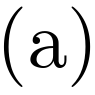
\includegraphics{figures/(a).png}

}

}

\end{minipage}%
%
\begin{minipage}[t]{0.01\linewidth}

{\centering 

~

}

\end{minipage}%
%
\begin{minipage}[t]{0.45\linewidth}

{\centering 

\raisebox{-\height}{

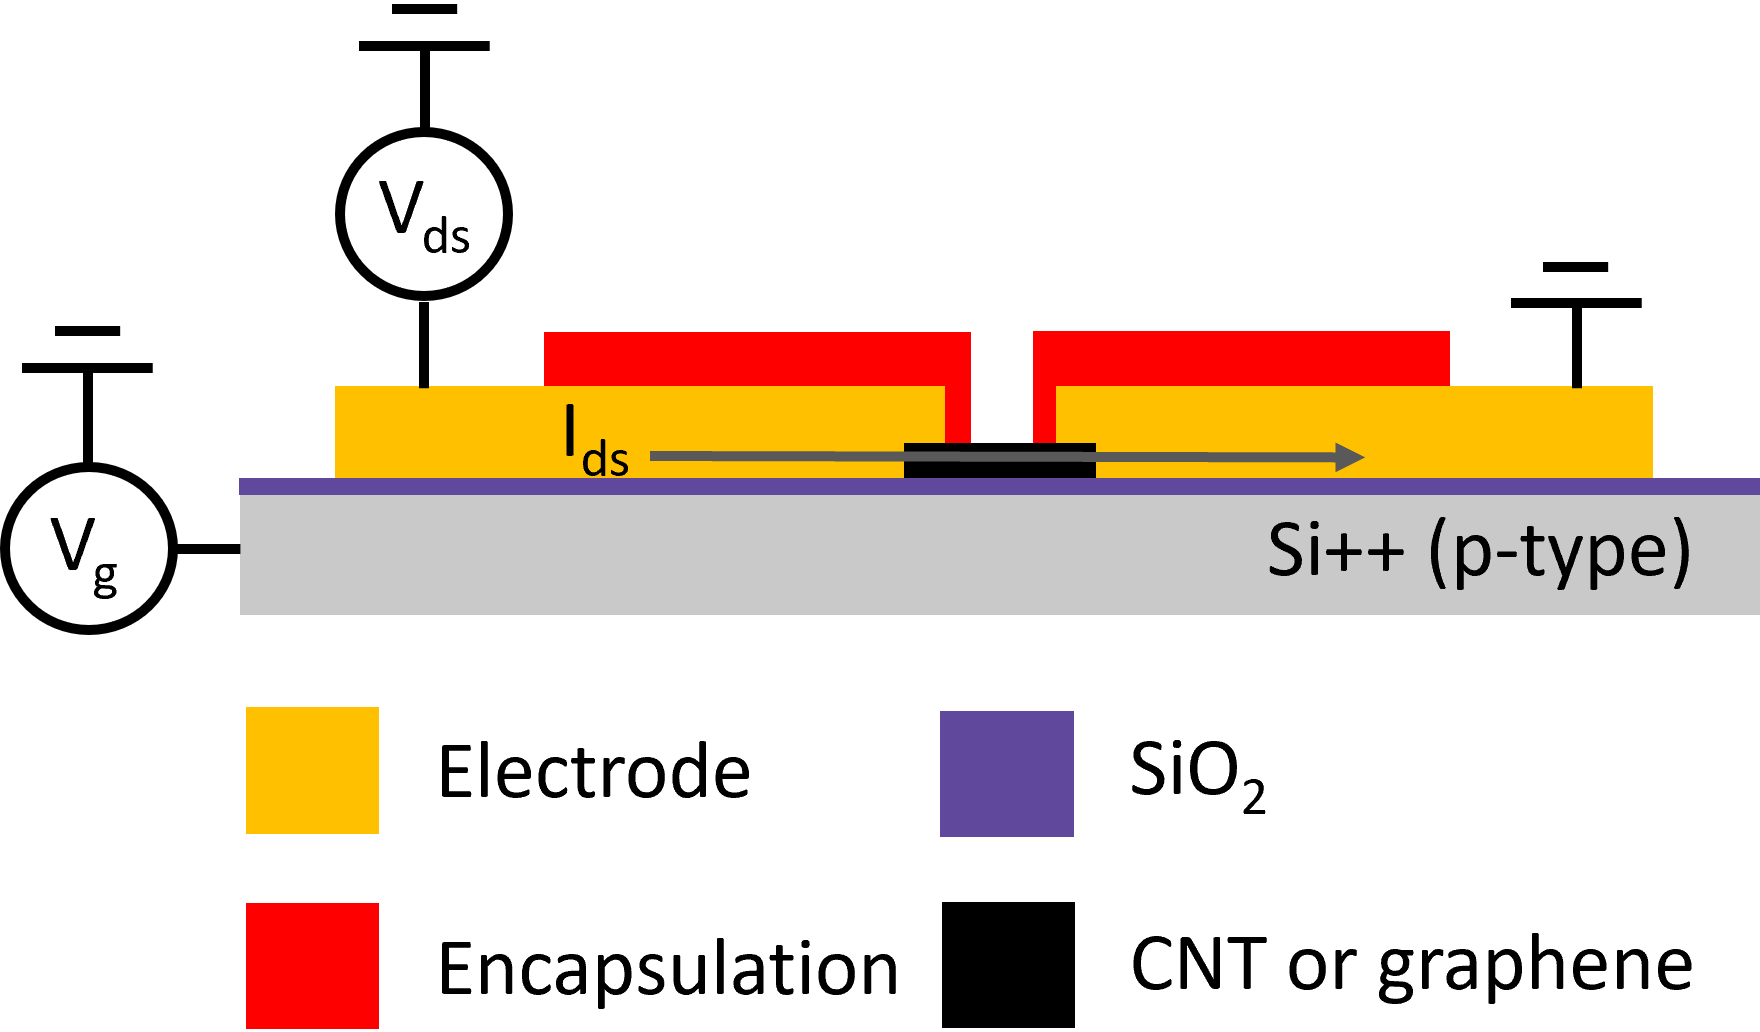
\includegraphics{figures/ch2/back-gate-schematic.png}

}

}

\end{minipage}%
%
\begin{minipage}[t]{0.01\linewidth}

{\centering 

~

}

\end{minipage}%
%
\begin{minipage}[t]{0.03\linewidth}

{\centering 

\raisebox{-\height}{

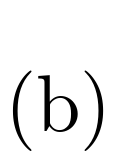
\includegraphics{figures/(b).png}

}

}

\end{minipage}%
%
\begin{minipage}[t]{0.01\linewidth}

{\centering 

~

}

\end{minipage}%
%
\begin{minipage}[t]{0.45\linewidth}

{\centering 

\raisebox{-\height}{

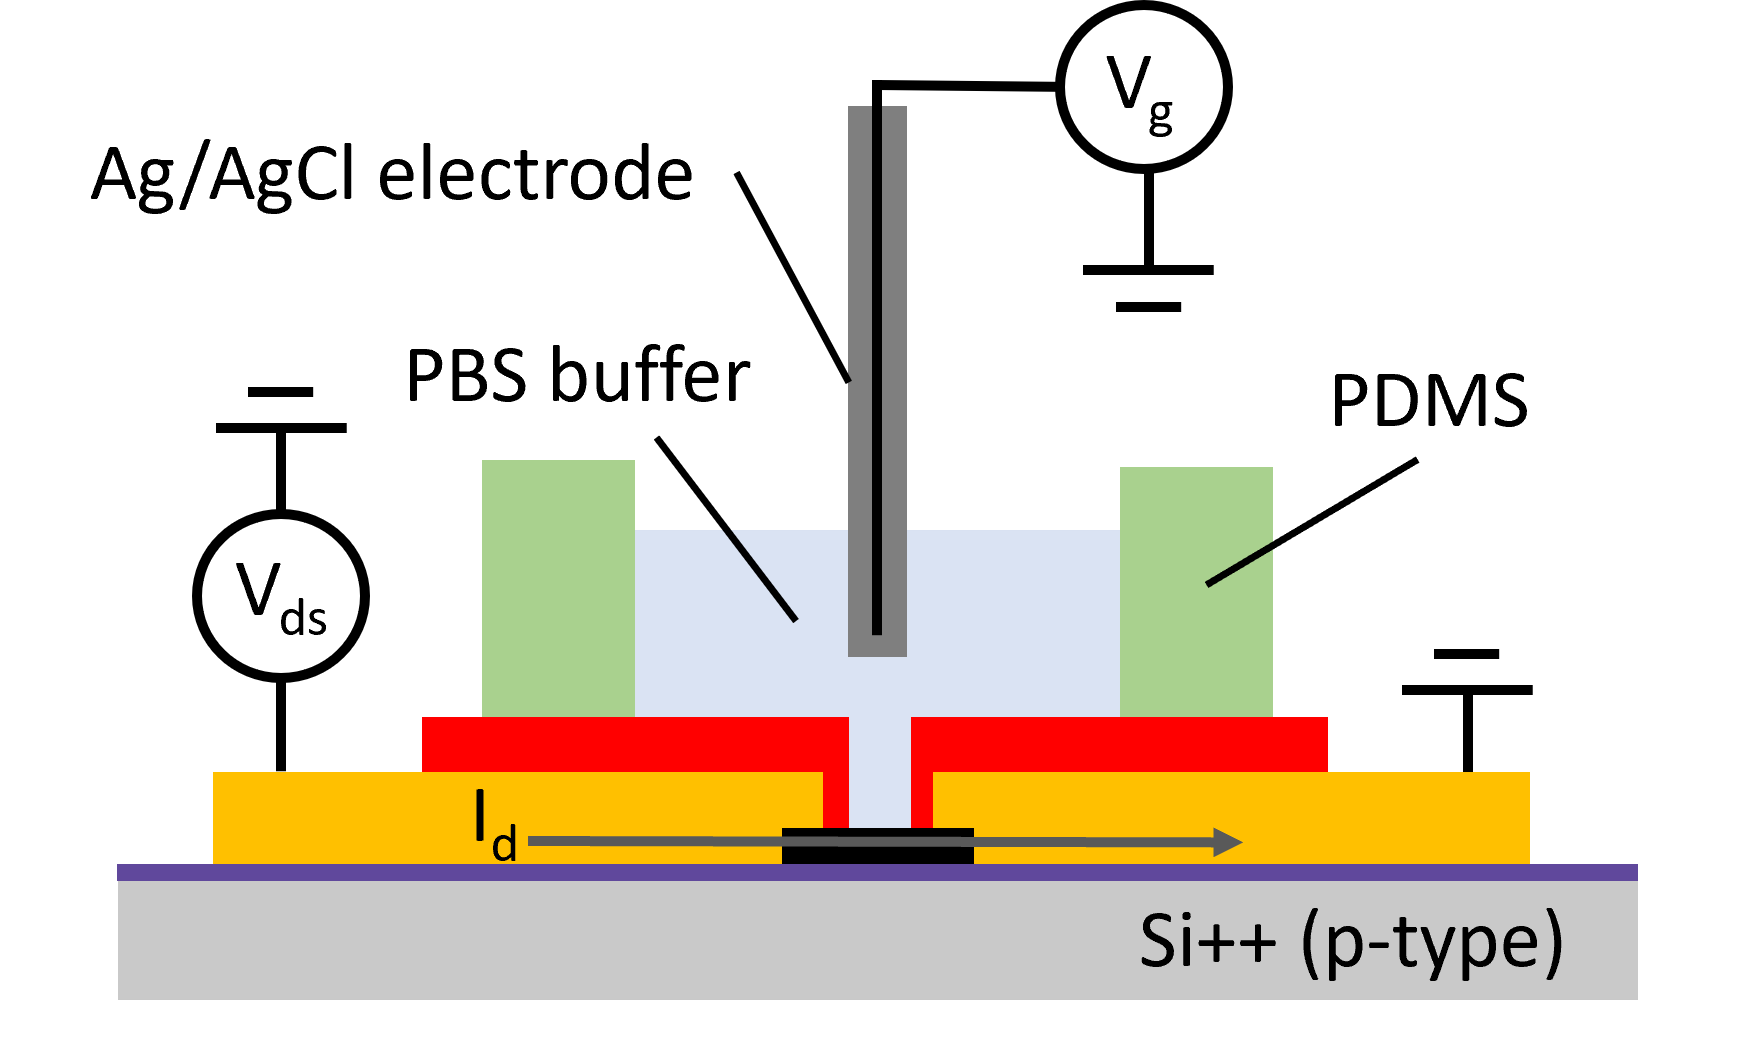
\includegraphics{figures/ch2/liquid-gate-schematic.png}

}

}

\end{minipage}%
%
\begin{minipage}[t]{0.01\linewidth}

{\centering 

~

}

\end{minipage}%

\caption{\label{fig-gating-schematics}Schematics (not to scale) showing
the side-view cross-section of a thin-film field-effect transistor in
both the (a) back-gated and (b) liquid-gated configuration. A graphene
monolayer or a carbon nanotube network is used as the transistor
thin-film.}

\end{figure}

\hypertarget{electrical-characterisation}{%
\subsection{Electrical
Characterisation}\label{electrical-characterisation}}

CNTFETs are traditionally \emph{p}-type transistors with positive charge
carriers \autocite{Martel1998,Kong2000}, while GFETs are ambipolar
\autocite{Ohno2010a}. Applying an gate voltage V\(_g\) to the gate of a
CNTFET or GFET increases, or decreases, the number of available charge
carriers, by bringing the relevant charge-carrying band closer to, or
further away from, the Fermi level of the channel \autocite{Sze2006}. An
example of both back-gated and liquid-gated transfer characteristics
from thin-film transistors are shown in
Figure~\ref{fig-gating-transfer}.

V\(_\textrm{ds}\) is the voltage between the source and drain electrodes
at either end of the semiconducting channel, and is known as the `drain
bias'. V\(_\textrm{g}\) is the potential beneath the gate, and is known
as the `gate bias'. The gate is insulated from the semiconducting
channel by an oxide layer. I\(_\textrm{d}\) is the current that flows
through the FET from the source to the drain. The current-voltage plot
of I\(_\textrm{d}\) against V\(_\textrm{g}\) is called the `transfer
characteristic curve' of the FET, while the I-V curve of
I\(_\textrm{d}\) against V\(_\textrm{ds}\) is called the `source-drain
characteristic curve' of the FET.

V\(_\textrm{g}\) is used to turn the FET on or off. A FET is known as
`normally-off' if at zero gate bias the channel conductance is very low,
and gate voltage must be applied to make the channel conductive.
Conversely, a FET is `normally-on' when the channel is conductive with
zero gate bias and must have a gate voltage applied to be turned off.
For \(p\)-type channel FETs, negative Vg brings the valence band closer
to the Fermi level, meaning more positive charge carriers are available.
Therefore these devices are made more conductive with a more negative
gate bias; an increase in V\(_\textrm{g}\) reduces I\(_\textrm{d}\). The
opposite is true for \(n\)-type channel devices, where a more positive
V\(_\textrm{g}\) brings the conduction band closer to the Fermi level,
meaning more negative charge carriers are available, making the device
more conductive. The increased availability of majority carriers in both
cases is known as `accumulation'.@fig-accumulation illustrates
accumulation in each situation.

\begin{figure}

{\centering 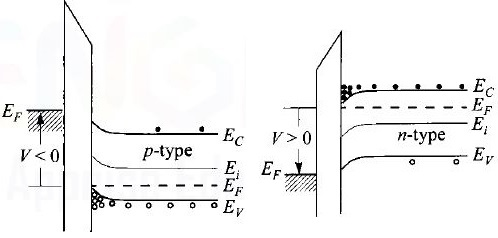
\includegraphics[width=0.5\textwidth,height=\textheight]{figures/ch2/accumulation.png}

}

\caption{\label{fig-accumulation}Energy band diagrams for a FET device
under accumulation conditions, where the left side of each diagram is
the gate region, while the right side is the channel region
\autocite{Sze2006}.}

\end{figure}

An important attribute of the transfer characteristic curve for all
thin-film FETs is the on-off current ratio. On-off current ratio is the
ratio of the current through a device when gated fully ``off'' with a
positive voltage, to the current through the device when gated fully
``on'' with a negative voltage \autocite{Zheng2017}. The off current in
an ambipolar FET can be defined as the minimum current during the
transfer sweep, where the majority carrier transitions from being holes
to electrons or vice versa. For example, the on current of the channel
shown in Figure~\ref{fig-gating-transfer} (b) is 741.5 nA, the off
current is 0.2 nA, and therefore the on-off ratio is \(\sim\) 3000. In
contrast, even when 10 V is applied, the backgated device shown in
Figure~\ref{fig-gating-transfer} (a) is never gated fully off.
Application of higher voltages to the gate result in significant leakage
currents through the gate, and can even result in irreversible breakdown
of the oxide layer \autocite{Sze2006}. Being able to traverse both on
and off regimes over a limited voltage interval is one of the many
advantages of the liquid-gated configuration.

In the linear I\(_\textrm{ds}\)-V\(_\textrm{ds}\) regime,
transconductance is given by dI\(_\textrm{ds}\)/dV\(_\textrm{g}\) ,
which gives a measure of the mobility of the charge carriers in the
device channel \autocite{Martel1998,Sze2006,Zheng2017}.

\begin{figure}

\begin{minipage}[t]{0.03\linewidth}

{\centering 

\raisebox{-\height}{

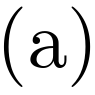
\includegraphics{figures/(a).png}

}

}

\end{minipage}%
%
\begin{minipage}[t]{0.01\linewidth}

{\centering 

~

}

\end{minipage}%
%
\begin{minipage}[t]{0.45\linewidth}

{\centering 

\raisebox{-\height}{

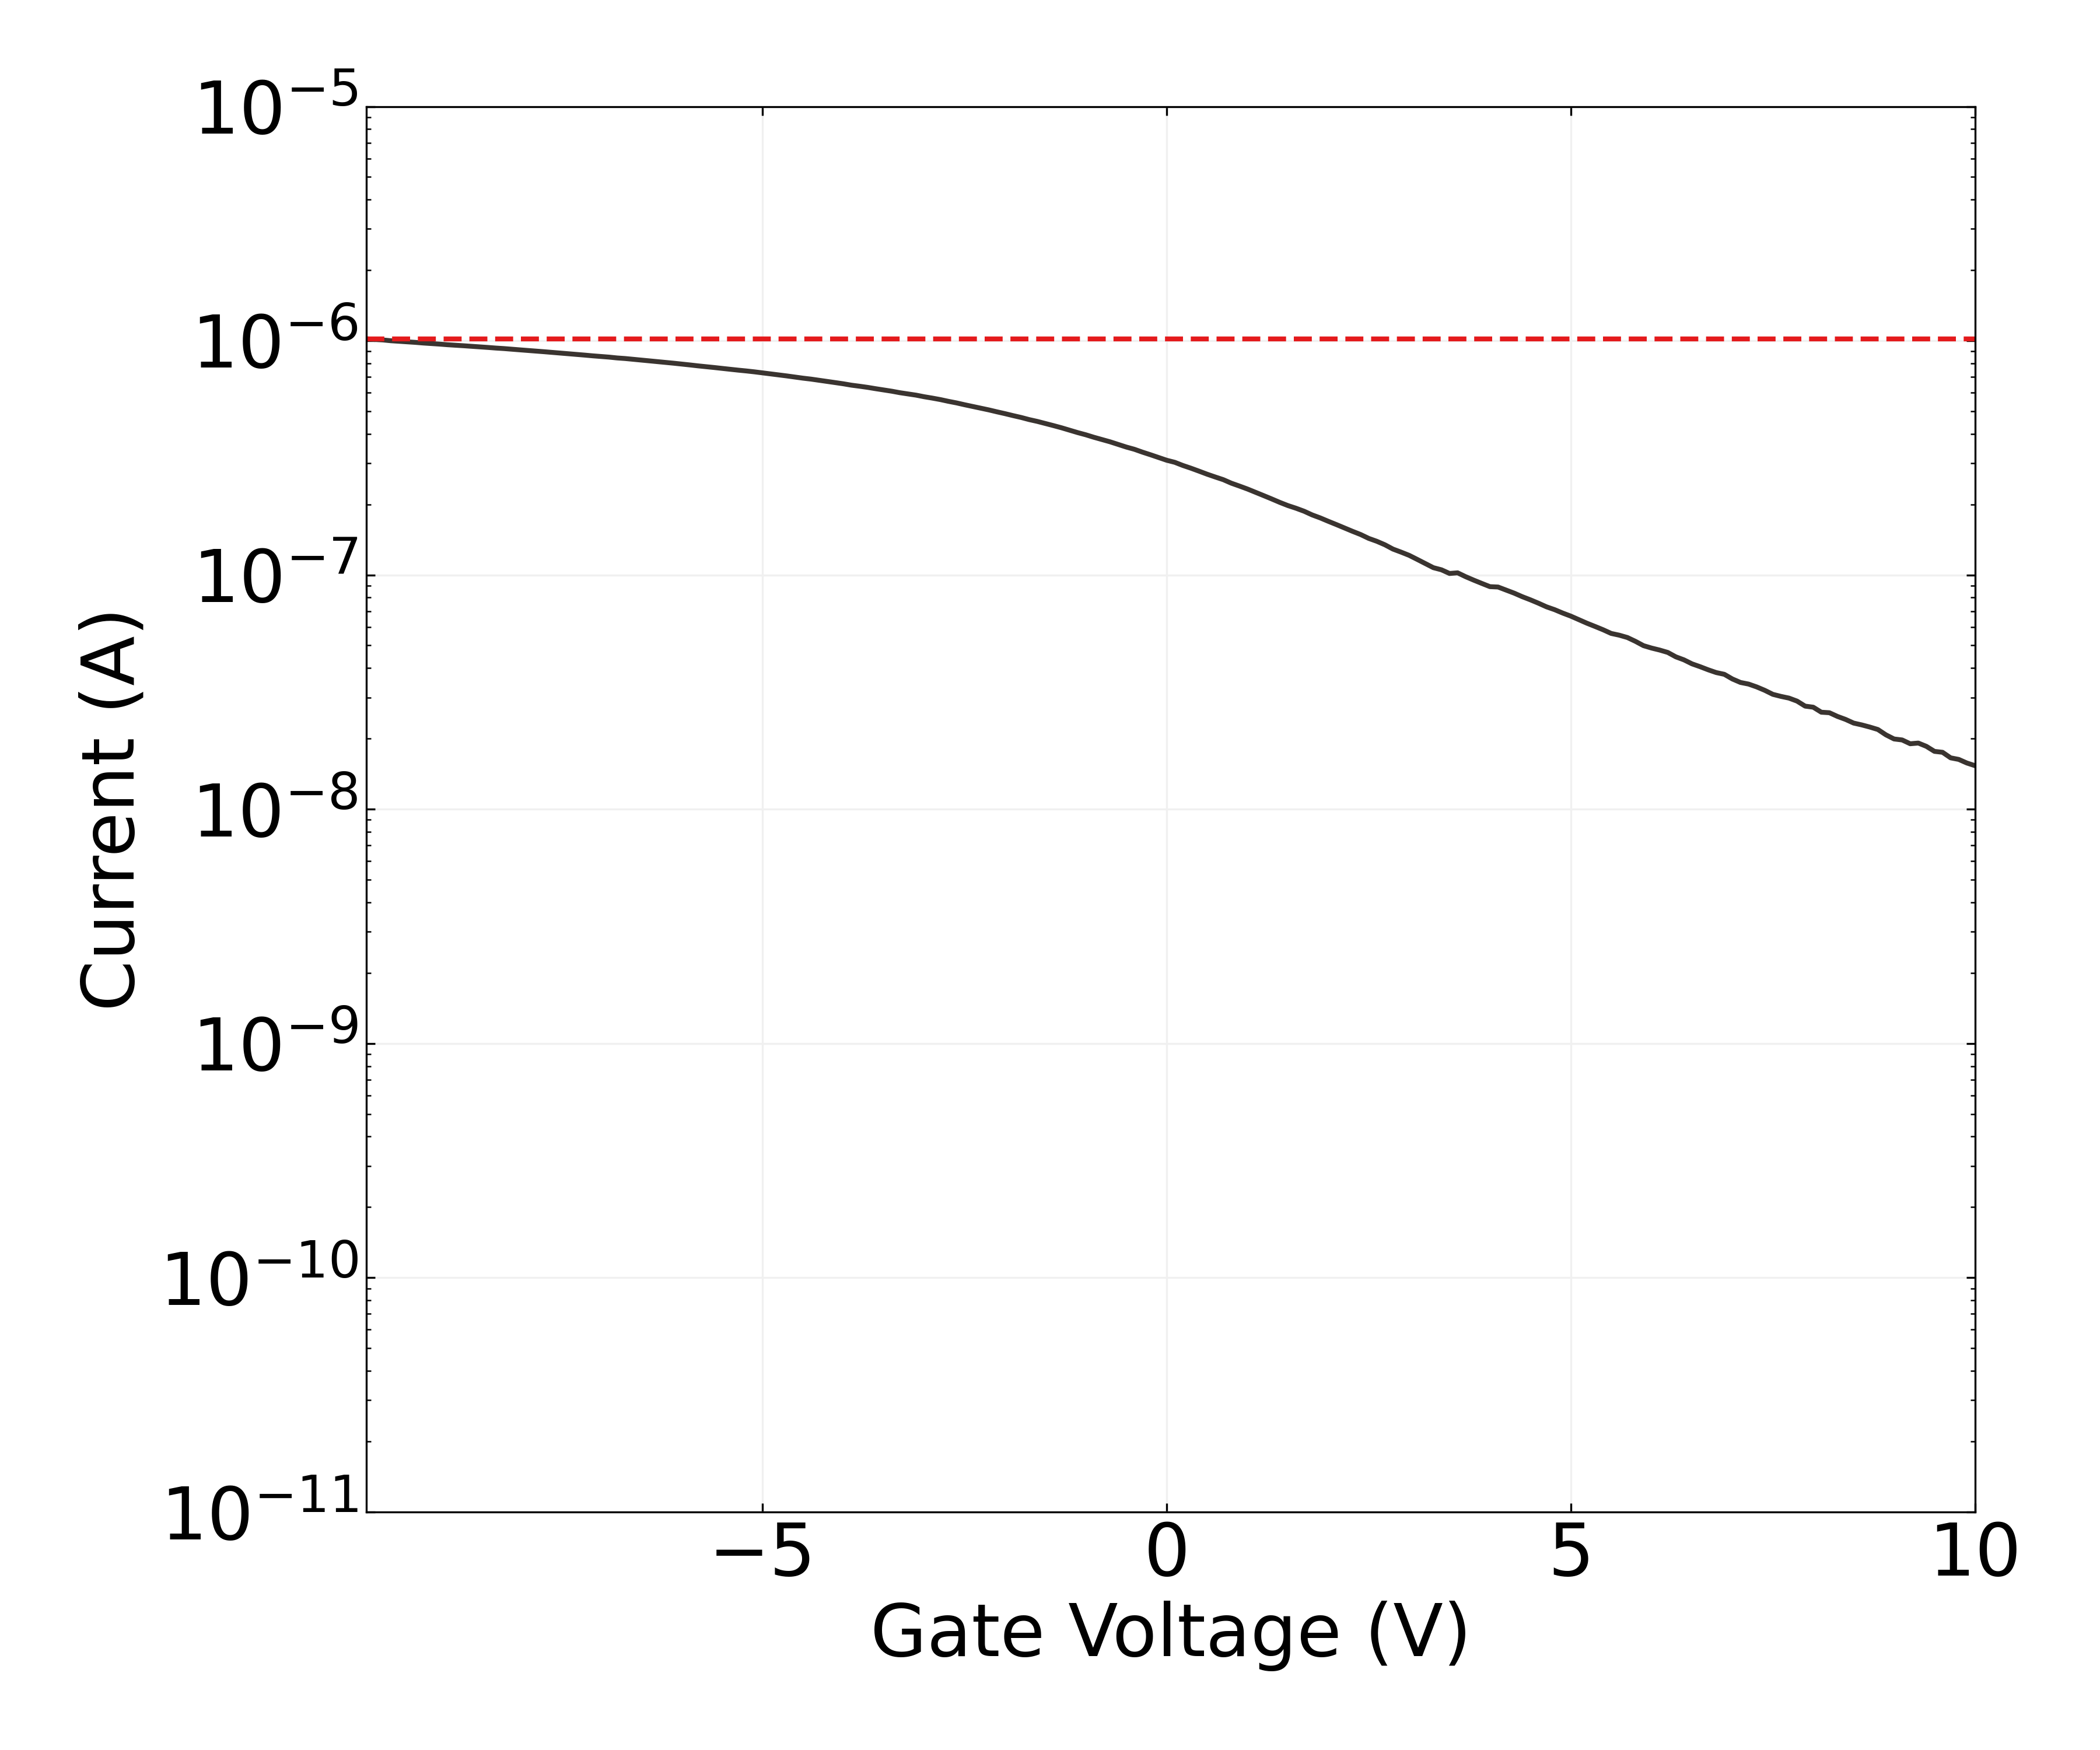
\includegraphics{figures/ch2/Q5C10ch5on_current.png}

}

}

\end{minipage}%
%
\begin{minipage}[t]{0.01\linewidth}

{\centering 

~

}

\end{minipage}%
%
\begin{minipage}[t]{0.03\linewidth}

{\centering 

\raisebox{-\height}{

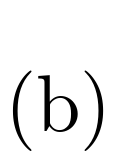
\includegraphics{figures/(b).png}

}

}

\end{minipage}%
%
\begin{minipage}[t]{0.01\linewidth}

{\centering 

~

}

\end{minipage}%
%
\begin{minipage}[t]{0.45\linewidth}

{\centering 

\raisebox{-\height}{

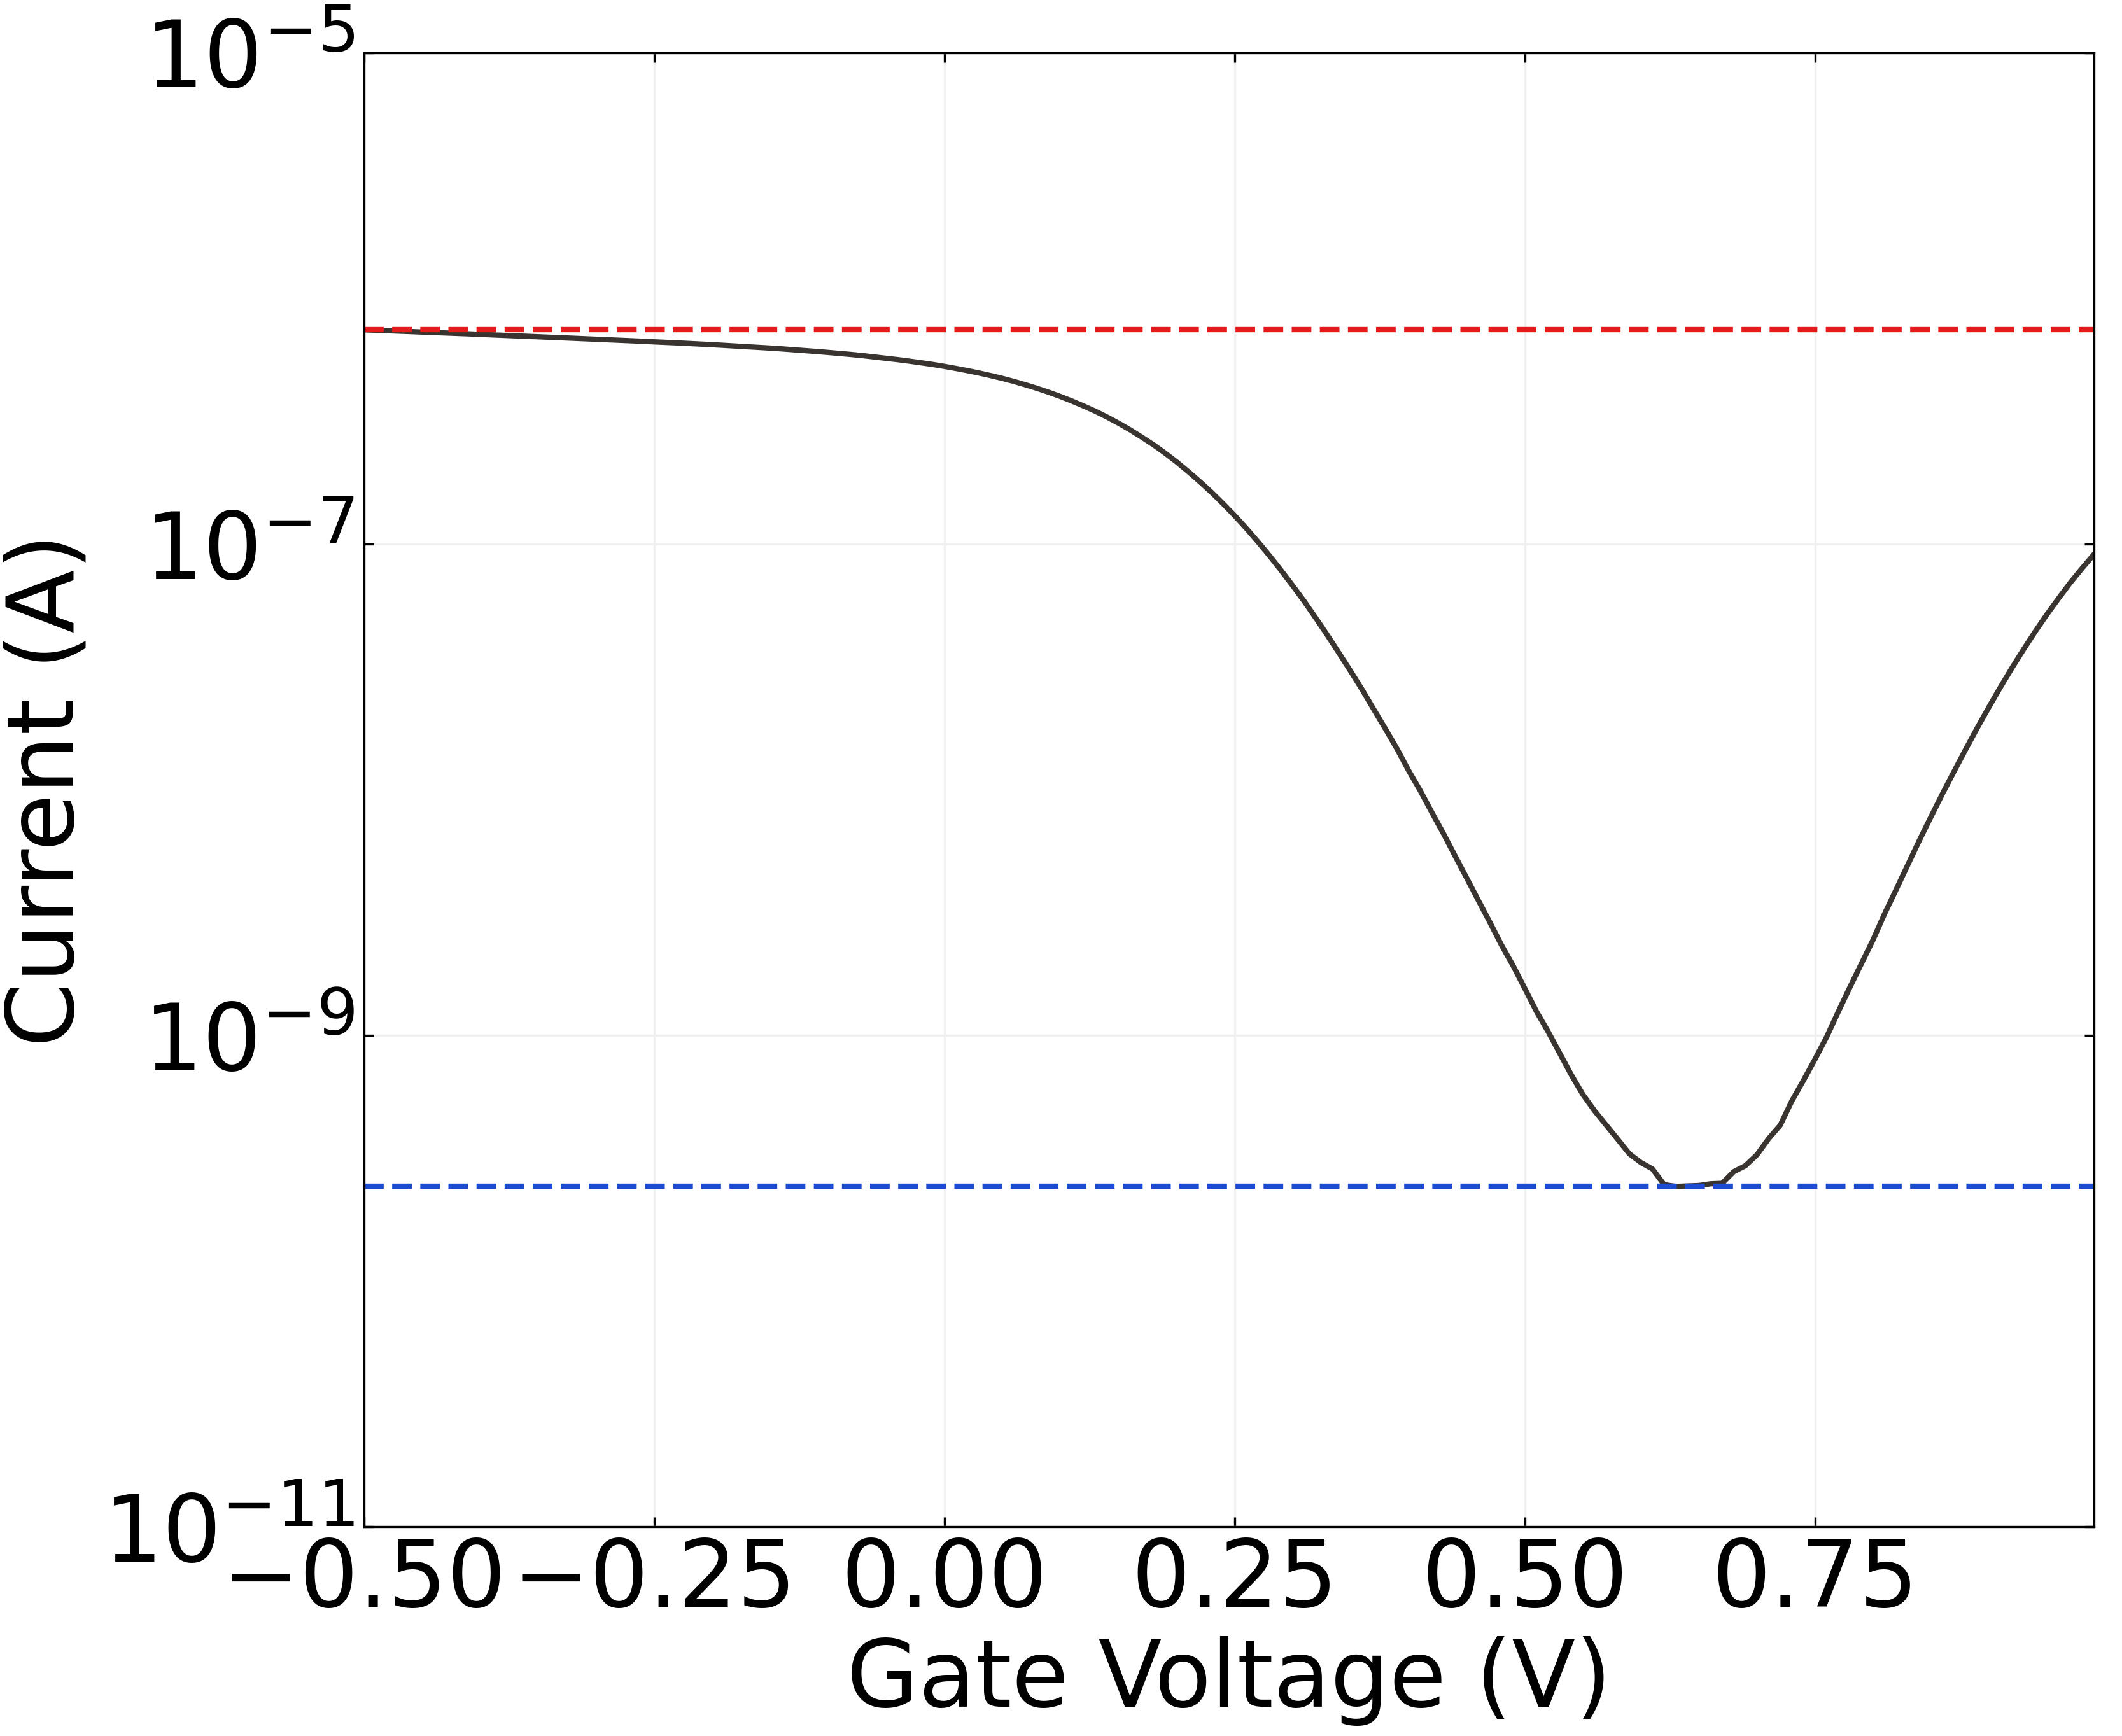
\includegraphics{figures/ch2/NTQ31C5ch1on_off_current.png}

}

}

\end{minipage}%
%
\begin{minipage}[t]{0.01\linewidth}

{\centering 

~

}

\end{minipage}%
\newline
\begin{minipage}[t]{0.03\linewidth}

{\centering 

\raisebox{-\height}{

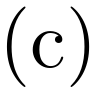
\includegraphics{figures/(c).png}

}

}

\end{minipage}%
%
\begin{minipage}[t]{0.01\linewidth}

{\centering 

~

}

\end{minipage}%
%
\begin{minipage}[t]{0.45\linewidth}

{\centering 

\raisebox{-\height}{

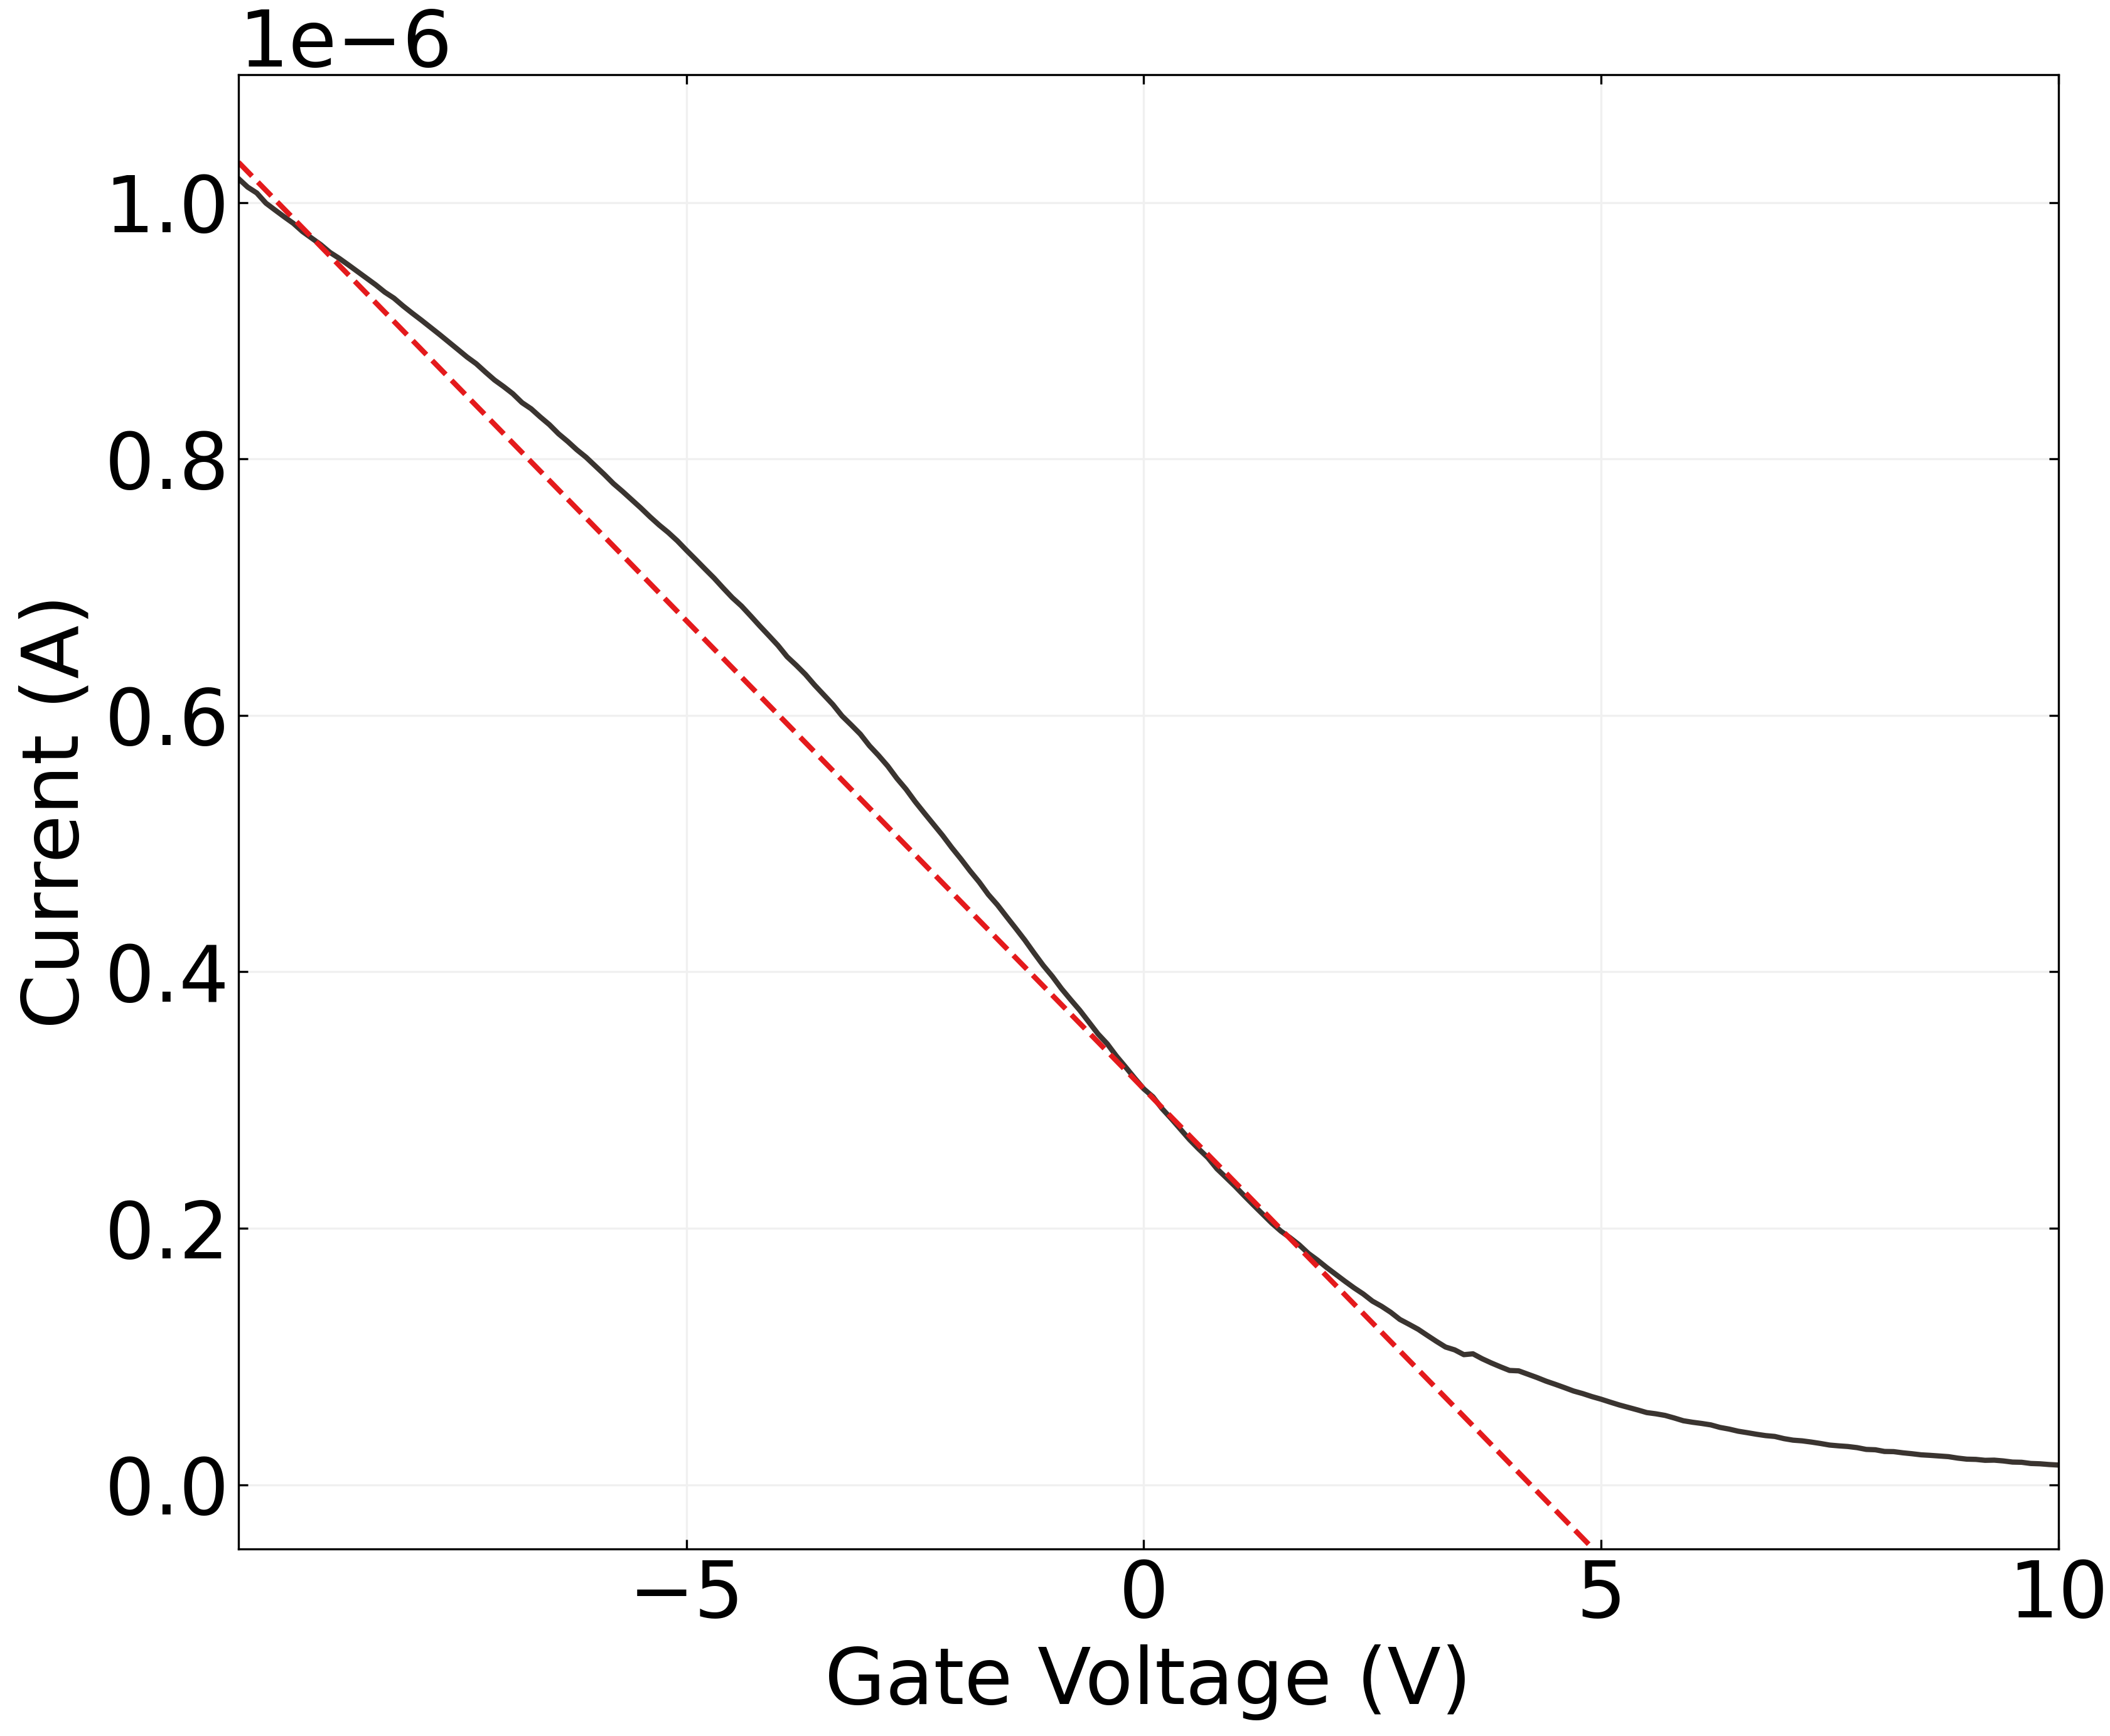
\includegraphics{figures/ch2/Q5C10ch5transconductance.png}

}

}

\end{minipage}%
%
\begin{minipage}[t]{0.01\linewidth}

{\centering 

~

}

\end{minipage}%
%
\begin{minipage}[t]{0.03\linewidth}

{\centering 

\raisebox{-\height}{

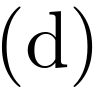
\includegraphics{figures/(d).png}

}

}

\end{minipage}%
%
\begin{minipage}[t]{0.01\linewidth}

{\centering 

~

}

\end{minipage}%
%
\begin{minipage}[t]{0.45\linewidth}

{\centering 

\raisebox{-\height}{

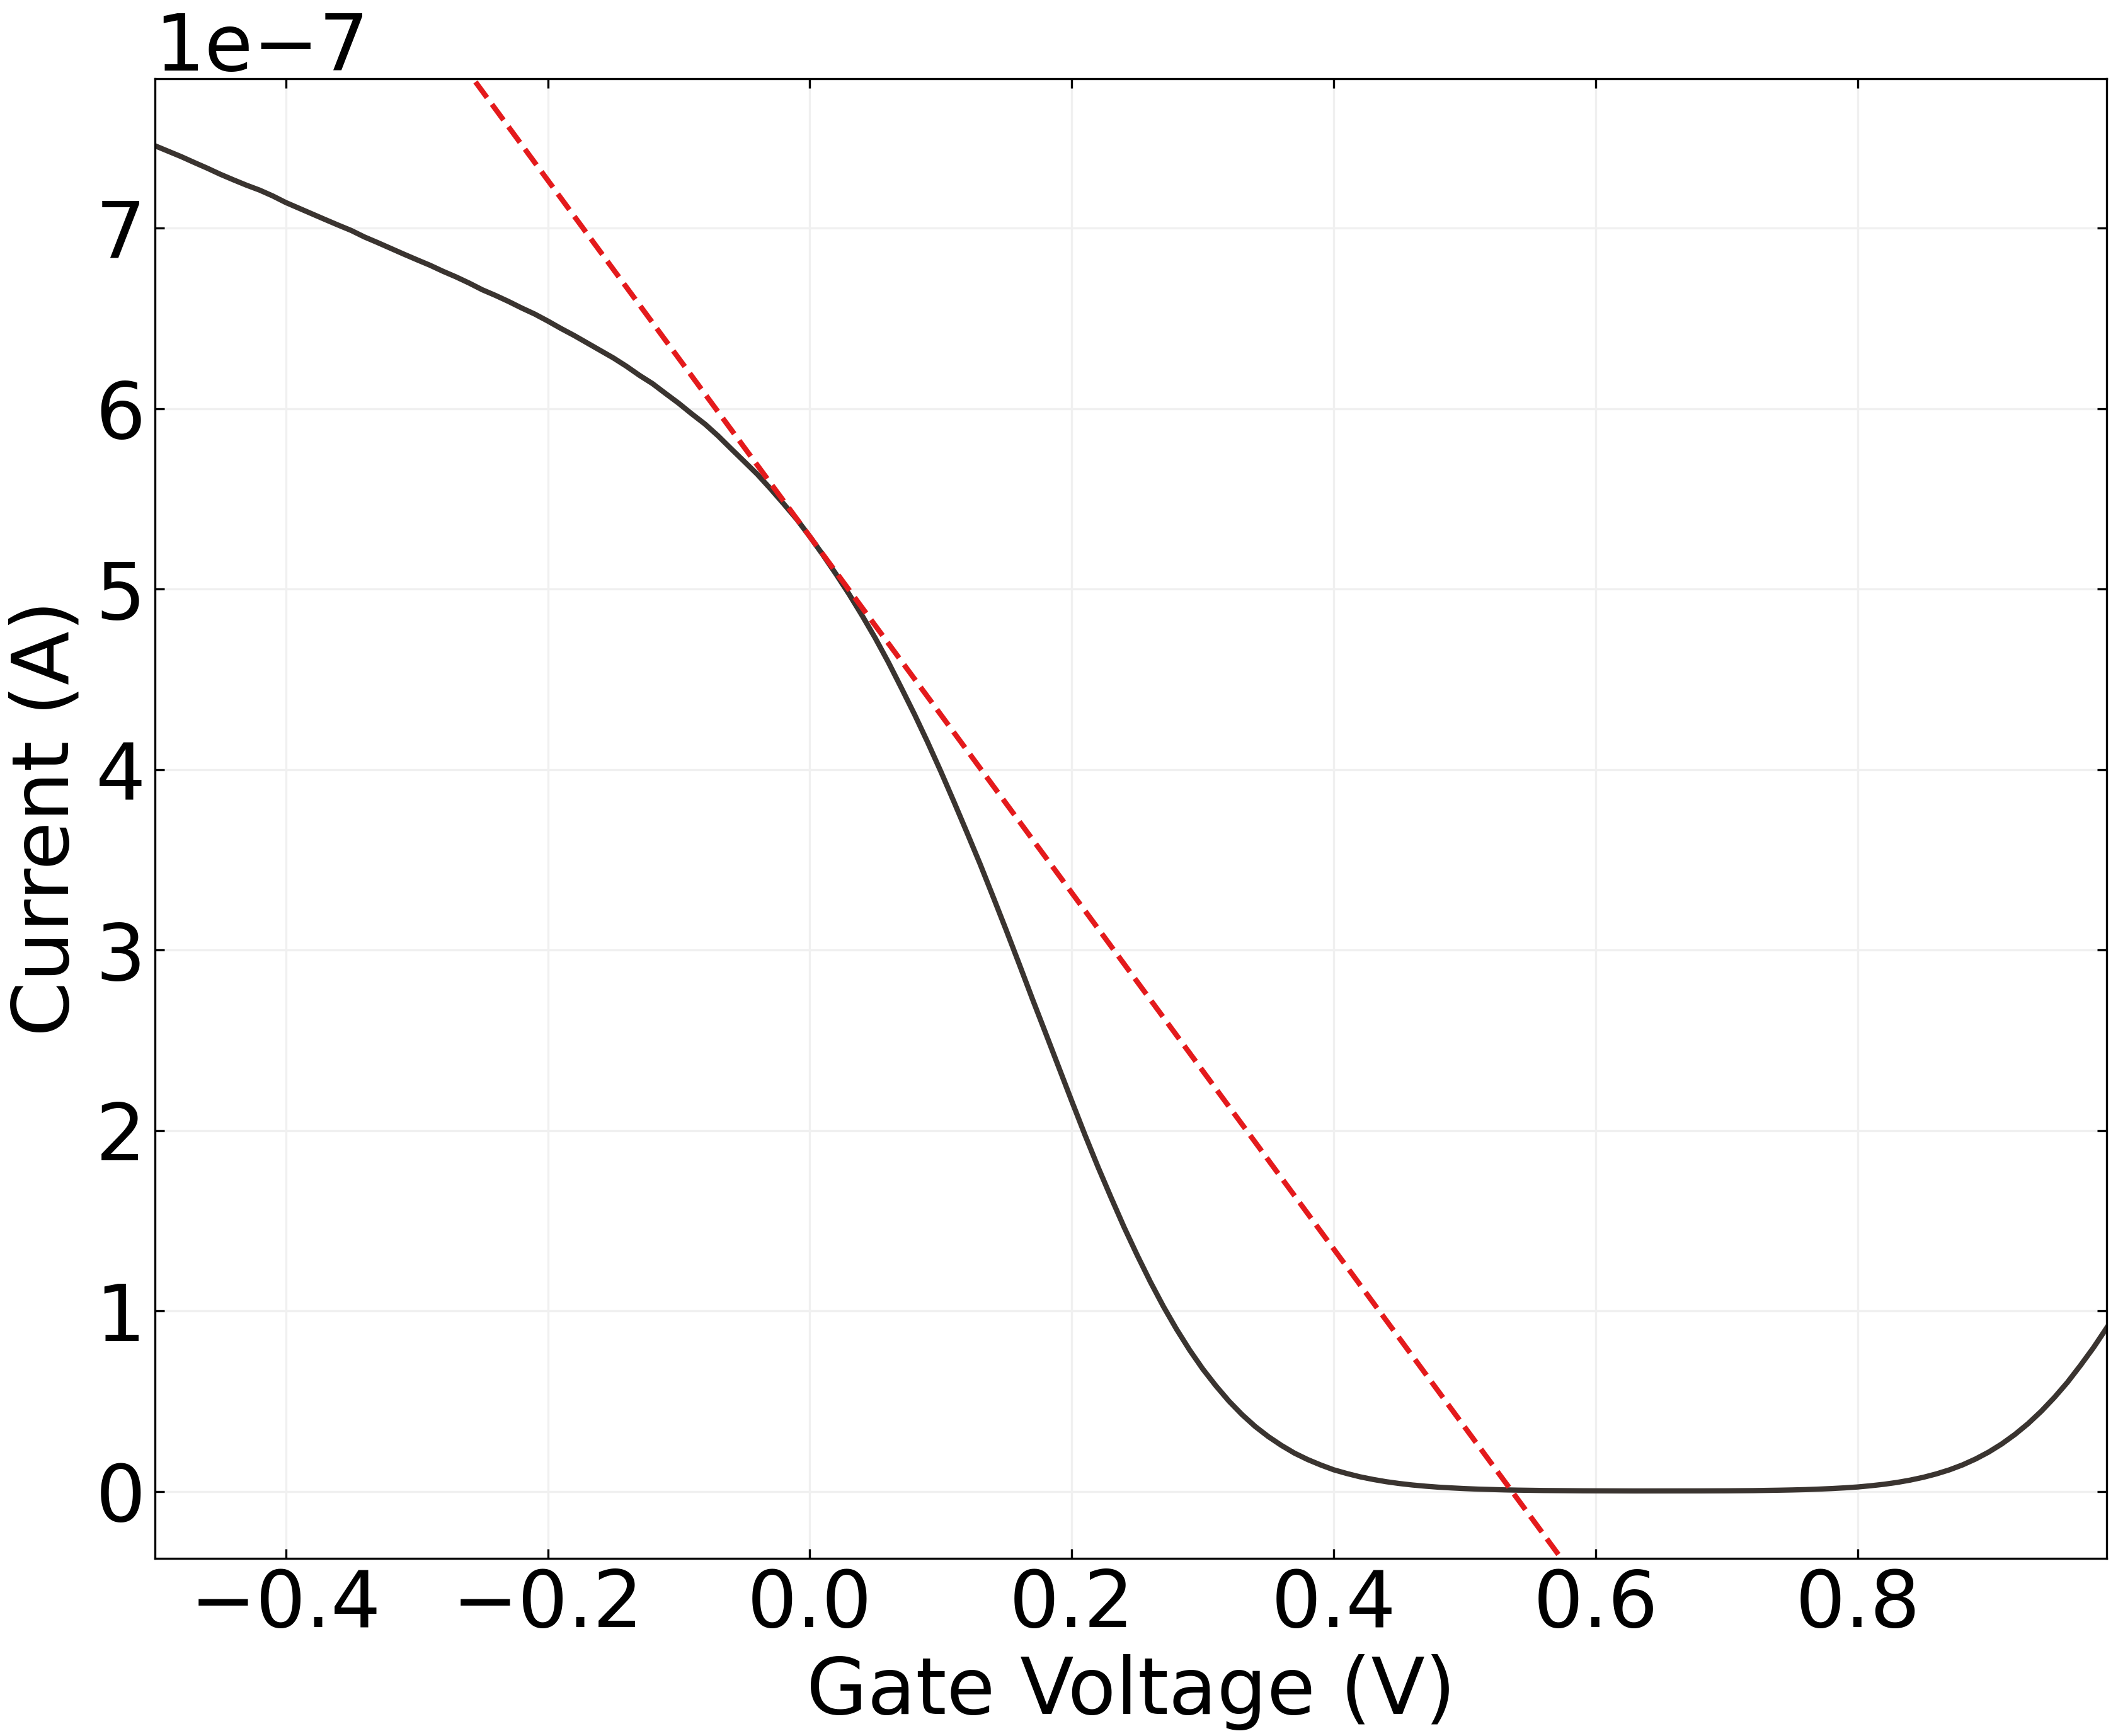
\includegraphics{figures/ch2/NTQ31C5ch1transconductance.png}

}

}

\end{minipage}%
%
\begin{minipage}[t]{0.01\linewidth}

{\centering 

~

}

\end{minipage}%

\caption{\label{fig-gating-transfer}Examples of field-effect transistor
transfer characteristics taken at V\(_\textrm{ds}\) = 100 mV from two
different device channels. A logarithmic scale is used in (a) and (b),
while a linear scale is used in (c) and (d). The device channel in (a)
and (c) was backgated while the device channel in (b) and (d) was
liquid-gated. The ``on'' current in (a) and (b) is shown with a red
horizontal line, while the ``off'' current in (b) is shown with a blue
horizontal line. The linear fit with gradient corresponding to
transconductance at V\(_\textrm{g}\) = 0 V is shown in (c) and (d) with
a dotted red line.}

\end{figure}

Channel carriers in a FET can be accelerated by a sufficiently high
gate-channel field into surmounting the insulating barrier between the
gate and channel. This is known as `breakdown'. The breakdown voltage
V\(_\textrm{b}\) gives an upper limit to the bias able to be applied
across the device without the device being destroyed. Percolation theory
can be used to explain breakdown. As energetic carriers pass through the
oxide, defects are created randomly. When these random defects are dense
enough to form a chain from the gate to the semiconductor, a short is
created and breakdown occurs. With decreased oxide thickness the the
required voltage for breakdown also decreases, due to increased carrier
tunnelling.

\hypertarget{current-sampling}{%
\subsection{Current Sampling}\label{current-sampling}}

It is important to account for the changes in current that occur during
a sensing run that are unrelated to sensing, and try to minimise these
changes as much as possible. These changes are due to a variety of
causes and can be categorised as various types of noise and baseline
drift. (1/f noise paper, heller paper)

\hypertarget{graphene-field-effect-transistors}{%
\section{Graphene Field-Effect
Transistors}\label{graphene-field-effect-transistors}}

\hypertarget{sec-electrical-characterisation-graphene}{%
\subsection{Electrical
Characterisation}\label{sec-electrical-characterisation-graphene}}

\begin{figure}

{\centering 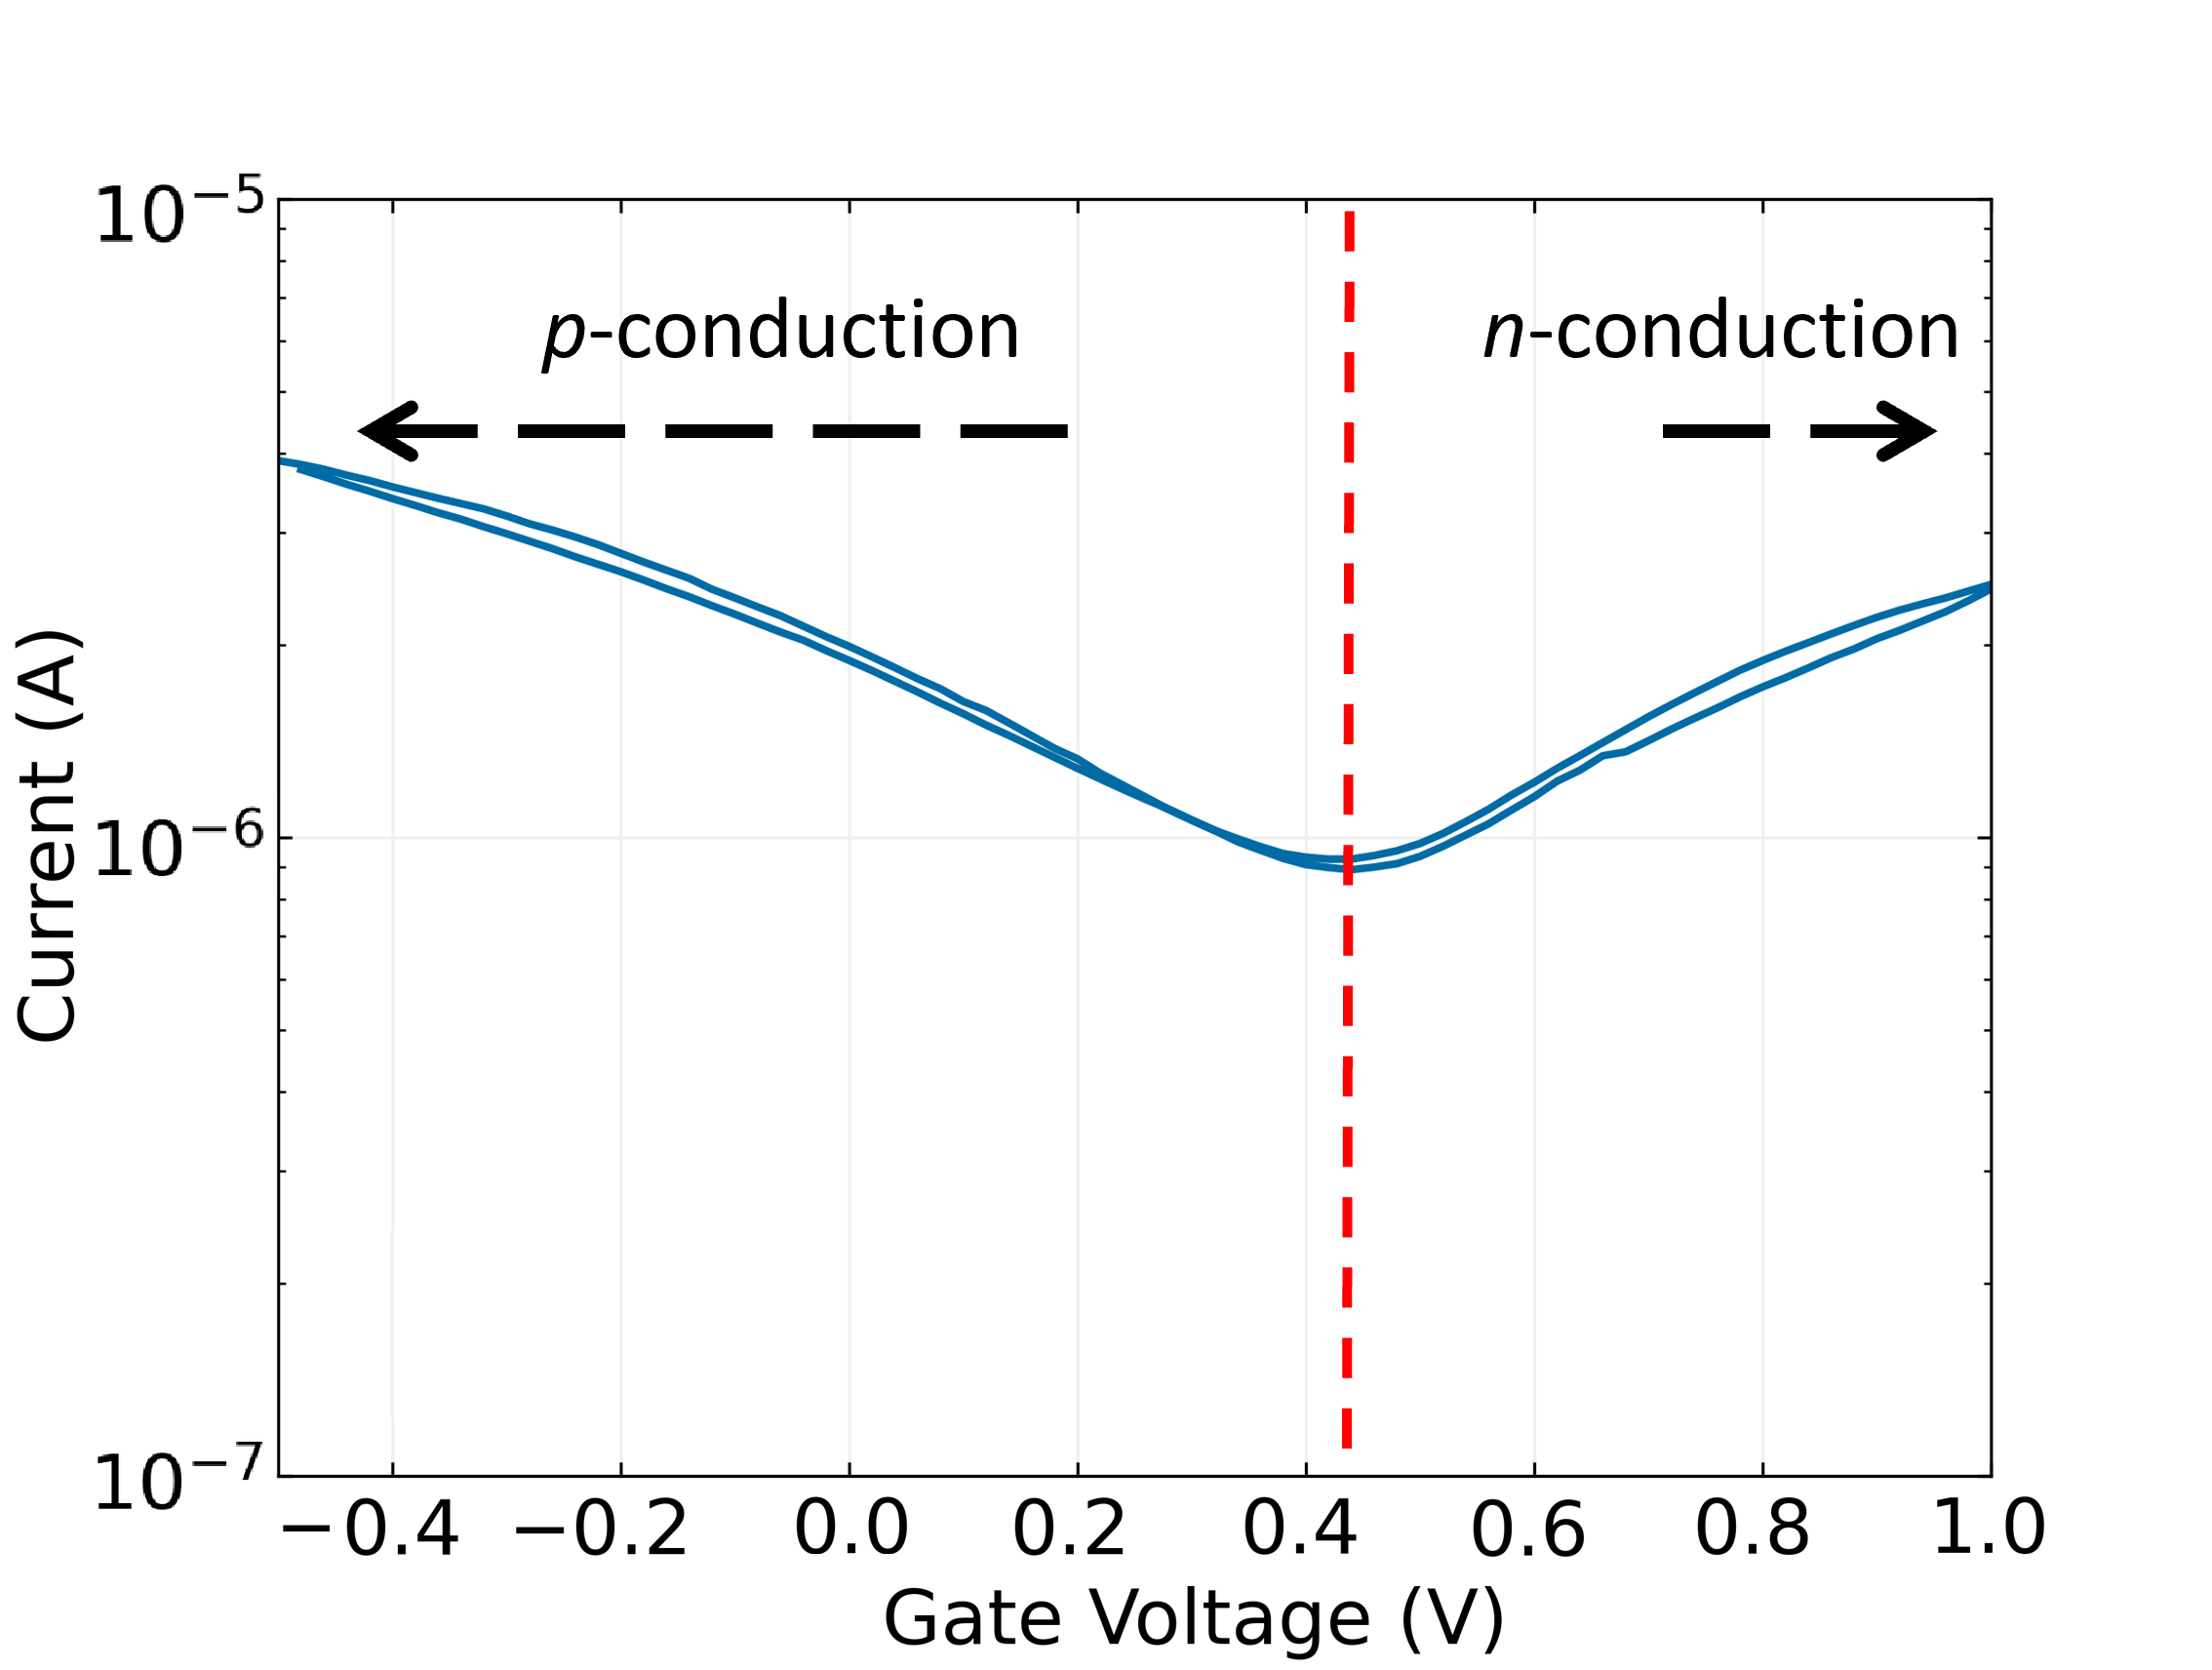
\includegraphics[width=0.6\textwidth,height=\textheight]{figures/ch2/Graphene_transfer.png}

}

\caption{\label{fig-linker-raman}Transfer characteristics of a graphene
field-effect transistor channel showing the regions of hole conduction
and electron conduction. The red dotted line indicates the Dirac point
voltage of the device channel.}

\end{figure}

As graphene FETs are ambipolar, they can never be gated into an `off'
regime. In normal operation of a GFET, the lowest voltage obtainable by
gating is known as the Dirac voltage \autocite{Murugathas2020}.

Quantative measurement of leftward shift in transfer curve Use minima of
curve in reverse sweep direction (more consistent than reading in
forward sweep direction) I compared the transfer characteristics after
then rinse steps to the pristine characteristics Transfer shifts where
current drops to zero are excluded (indicates delamination/damage to
channel)

\hypertarget{random-network-carbon-nanotube-field-effect-transistors}{%
\section{Random-Network Carbon Nanotube Field-Effect
Transistors}\label{random-network-carbon-nanotube-field-effect-transistors}}

\hypertarget{composition-and-chirality}{%
\subsection{Composition and Chirality}\label{composition-and-chirality}}

A single-walled carbon nanotube (SWCNT) consists of a graphene sheet, a
flat carbon lattice with hexagonal cells, rolled up into a cylinder.
Since their discovery in 1991, a wide range of device applications for
carbon nanotubes (CNTs) have been proposed, based on CNTs being highly
sensitive to their environment
\autocite{Iijima1991,Battie2010,Boyd2014,Chen2019}. This high
sensitivity is due to the high surface-to-volume ratio of the CNTs,
which maximises the exposure of this electrically sensitive structure to
its surroundings \autocite{Battie2010}. SWCNT-based devices consume
little power, operate quickly and are flexible \autocite{Chen2019}.
Nanotubes in a network can have semiconducting characteristics (s-CNTs)
or metallic characteristics (m-CNTs), depending on their chirality
\autocite{Martel1998,Kong2000}. A single CNT will therefore have
different properties than a network of CNTs, where the individual
electrical properties of the CNT tubes are averaged out across the
network \autocite{Battie2010}.

\hypertarget{network-morphology}{%
\subsection{Network Morphology}\label{network-morphology}}

\hypertarget{sec-electrical-characterisation-CNT}{%
\subsection{Electrical
Characterisation}\label{sec-electrical-characterisation-CNT}}

\begin{figure}

\begin{minipage}[t]{0.03\linewidth}

{\centering 

\raisebox{-\height}{

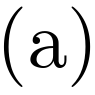
\includegraphics{figures/(a).png}

}

}

\end{minipage}%
%
\begin{minipage}[t]{0.01\linewidth}

{\centering 

~

}

\end{minipage}%
%
\begin{minipage}[t]{0.45\linewidth}

{\centering 

\raisebox{-\height}{

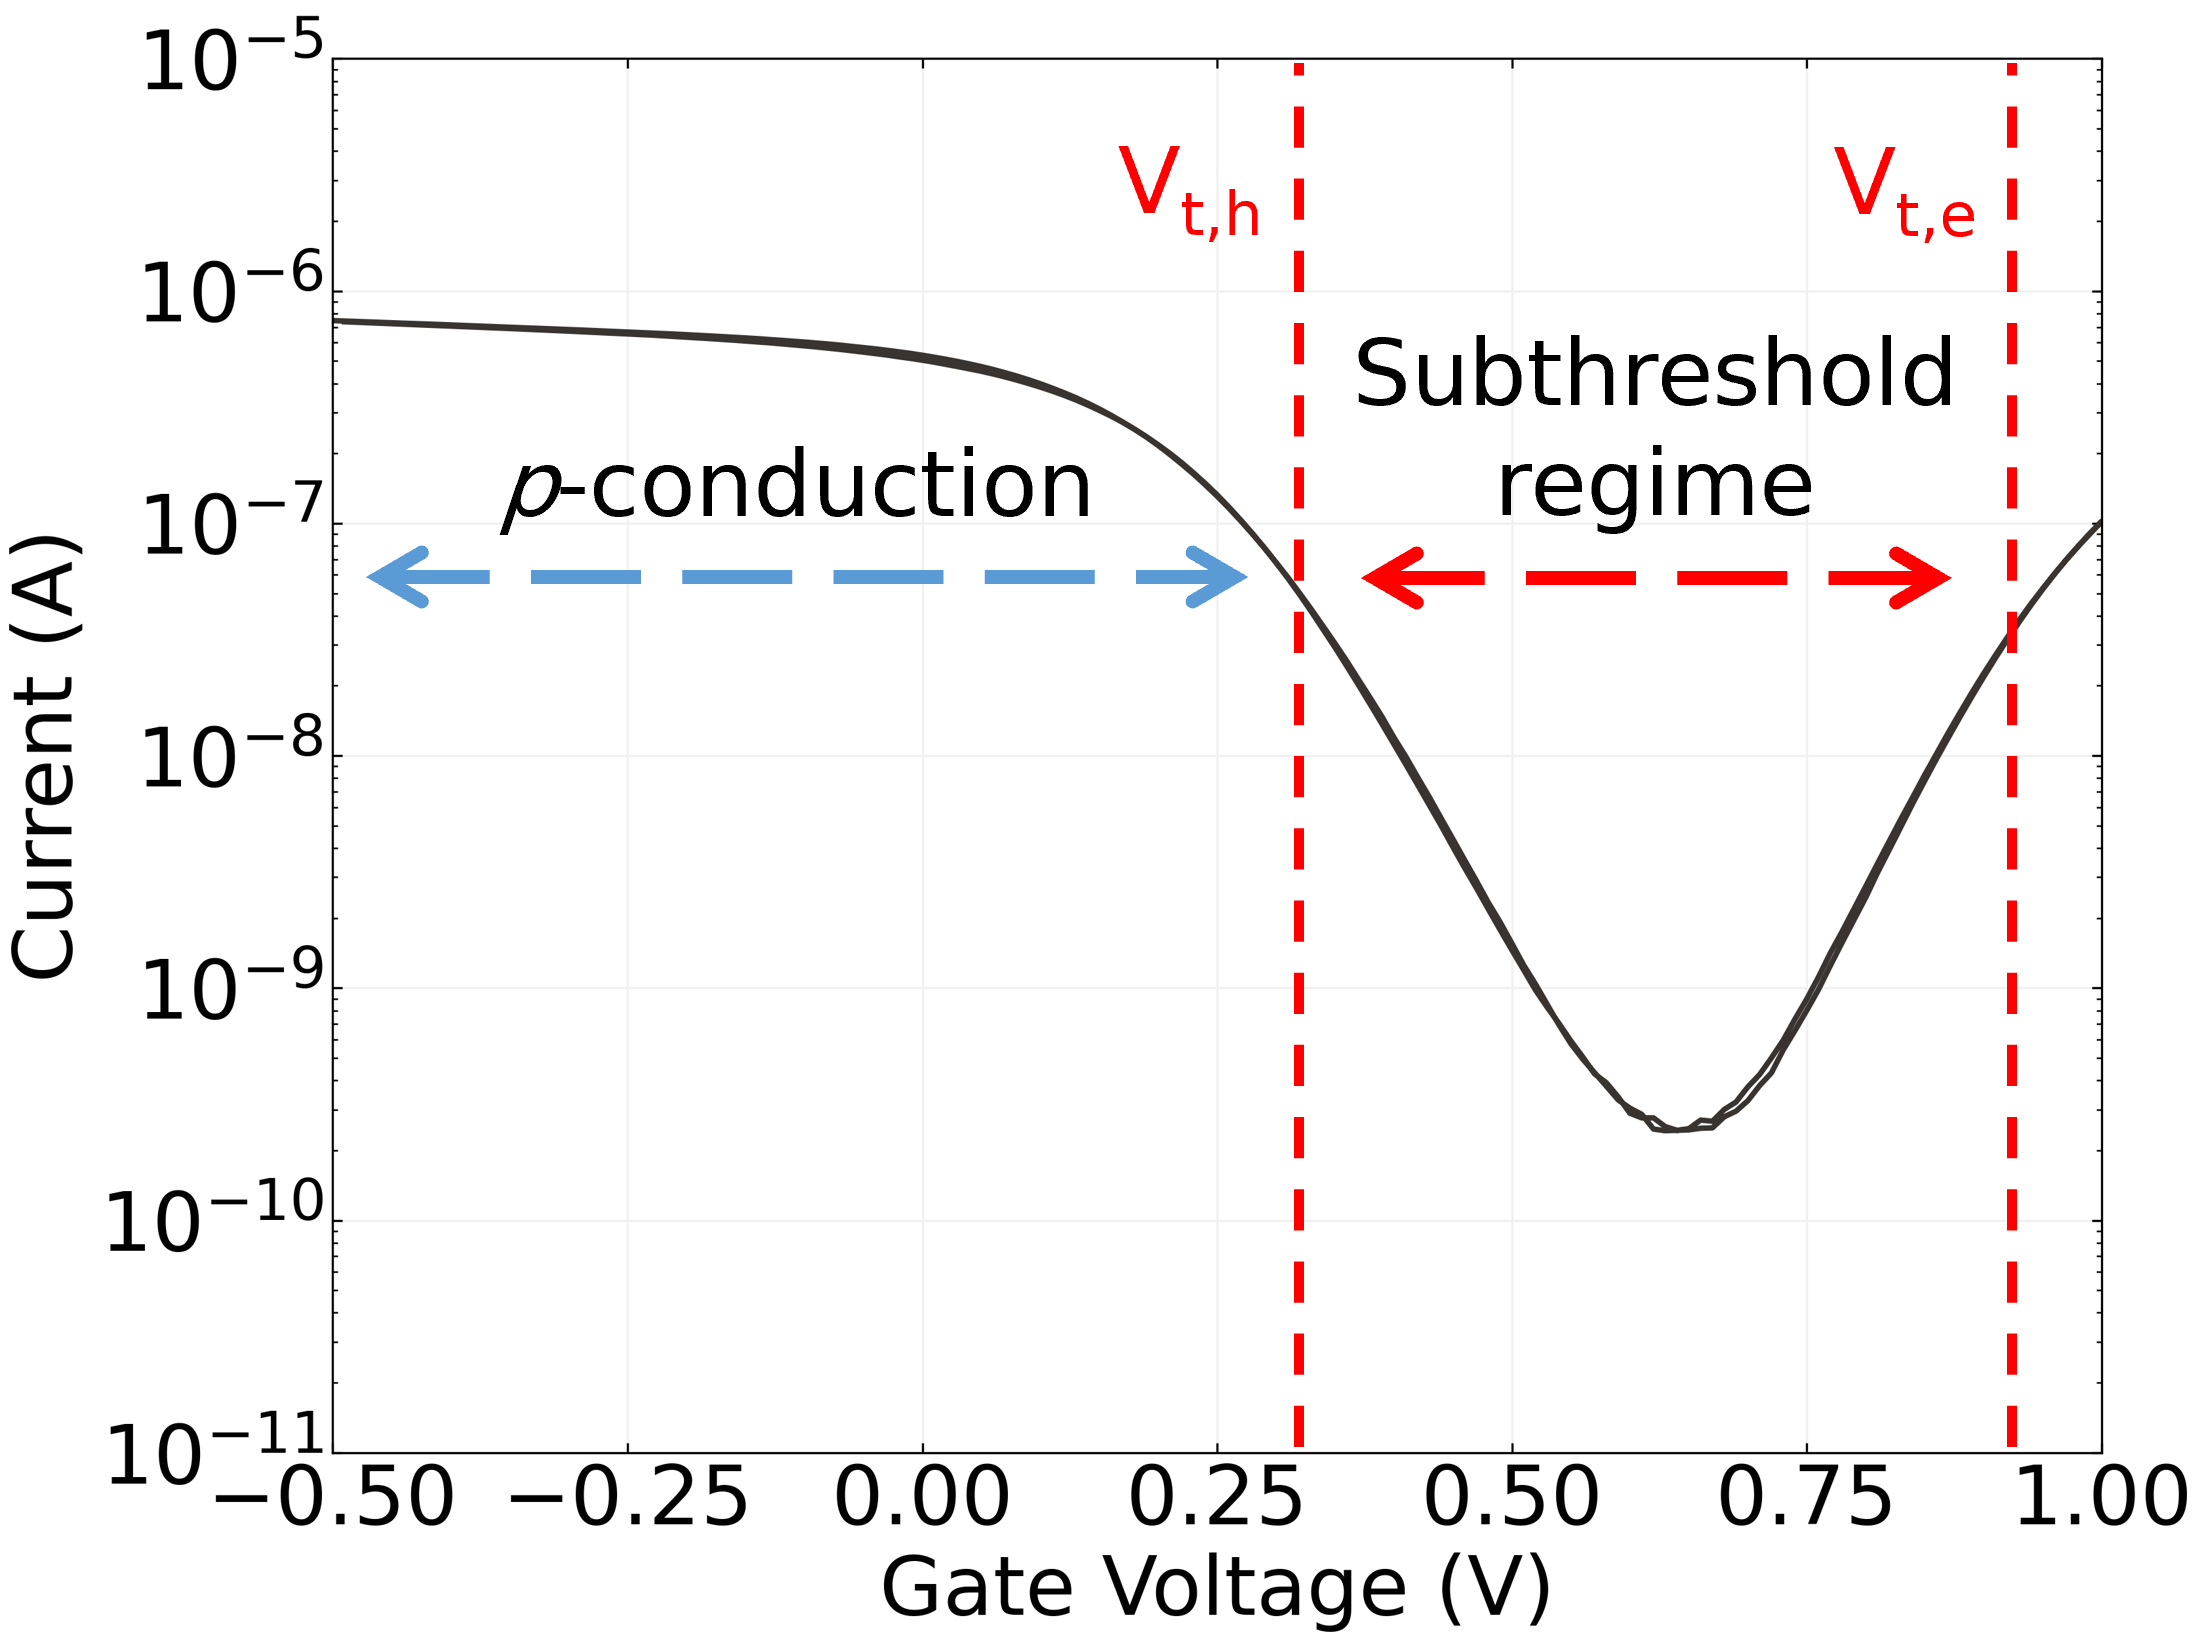
\includegraphics{figures/ch2/CNT_transfer_1.png}

}

}

\end{minipage}%
%
\begin{minipage}[t]{0.01\linewidth}

{\centering 

~

}

\end{minipage}%
%
\begin{minipage}[t]{0.03\linewidth}

{\centering 

\raisebox{-\height}{

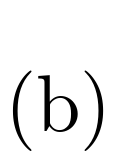
\includegraphics{figures/(b).png}

}

}

\end{minipage}%
%
\begin{minipage}[t]{0.01\linewidth}

{\centering 

~

}

\end{minipage}%
%
\begin{minipage}[t]{0.45\linewidth}

{\centering 

\raisebox{-\height}{

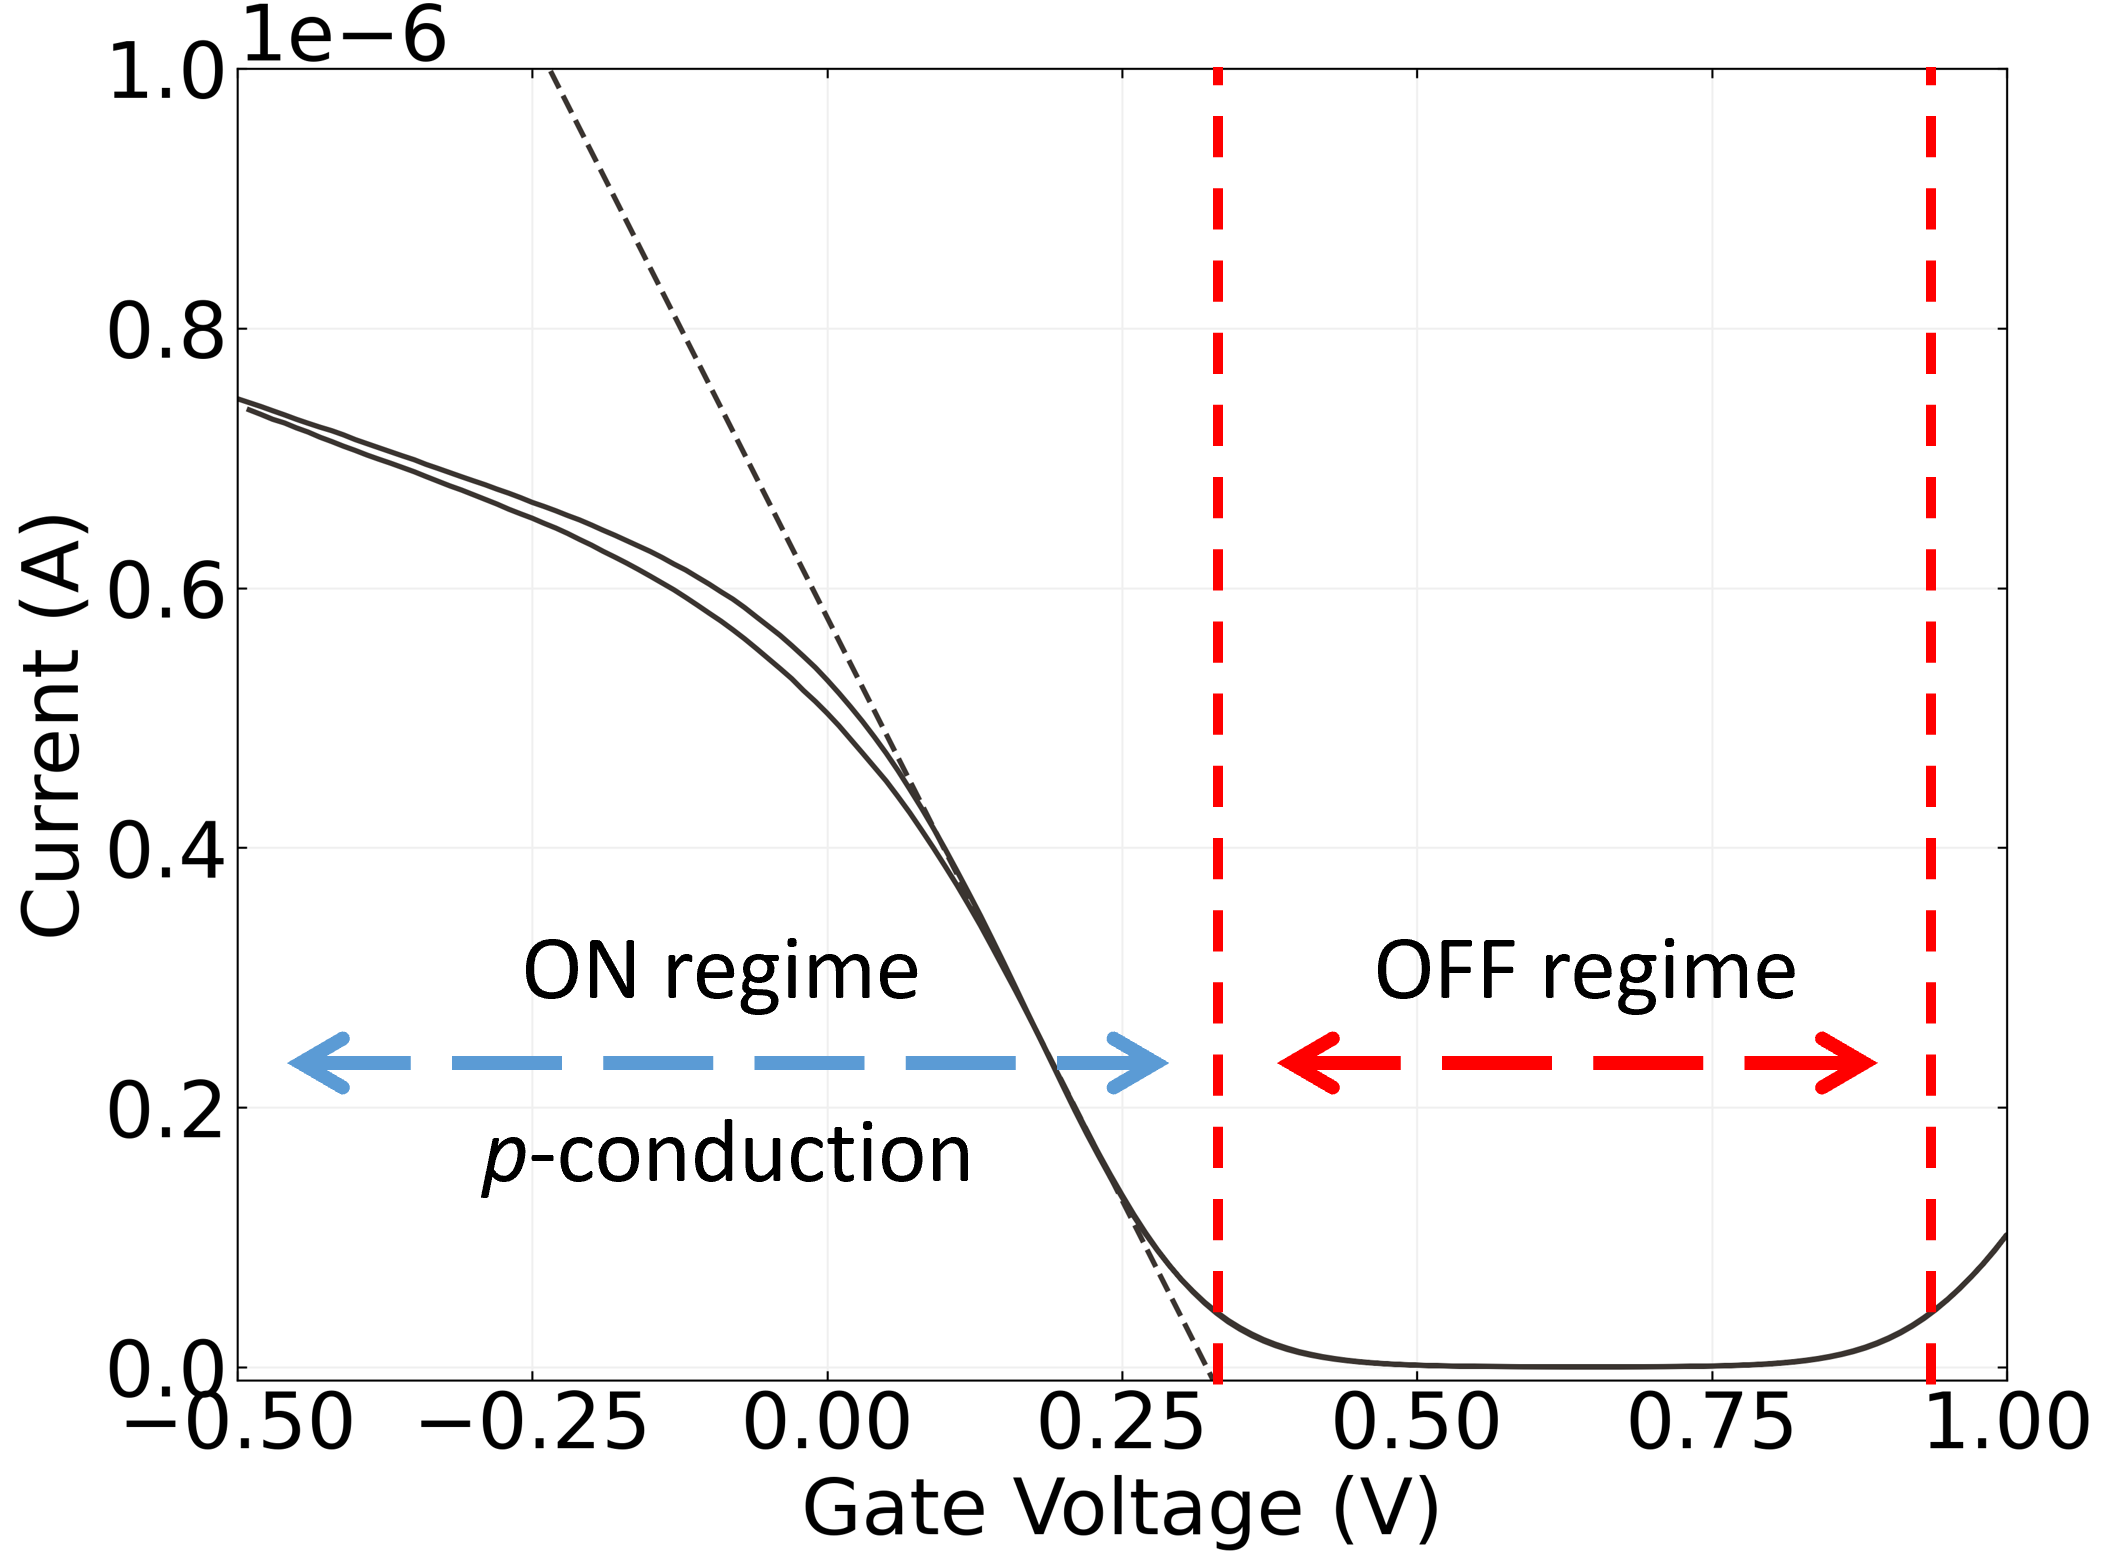
\includegraphics{figures/ch2/CNT_transfer_2.png}

}

}

\end{minipage}%
%
\begin{minipage}[t]{0.01\linewidth}

{\centering 

~

}

\end{minipage}%

\caption{\label{fig-literature-characteristics}Transfer characteristics
of a single carbon nanotube network field-effect transistor channel,
using a logarithmic scale in (a) and using a linear scale in (b) to
emphasise different features of the same dataset. The subthreshold slope
is shown with a black dotted line, while the threshold voltages are
shown with red dotted lines. The ON and OFF regimes are also indicated
on both figures.}

\end{figure}

\hypertarget{threshold-voltage}{%
\subsubsection*{Threshold Voltage}\label{threshold-voltage}}
\addcontentsline{toc}{subsubsection}{Threshold Voltage}

The threshold voltage is the voltage required to fully deplete the
device channel of charge carriers \autocite{Martel1998}. It can be
estimated by extrapolating the linear part of the transfer
characteristics of a device to the V\(_\textrm{g}\) axis.

The FET turns on at the `threshold voltage', V\(_\textrm{g}\) =
V\(_\textrm{t}\). For the \(p\)-type FET, when V\(_\textrm{g}\)
\textgreater{} V\(_\textrm{t}\), I\(_\textrm{d}\) increases linearly.

After decreasing past V\(_\textrm{t}\), I\(_\textrm{d}\) stays constant
at its `on' value I\(_\textrm{ON}\). The ratio of I\(_\textrm{ON}\) to
the I\(_\textrm{OFF}\) current is known as the FET device's `on-off
ratio', I\(_\textrm{ON}\)/I\(_\textrm{OFF}\). The threshold voltage can
be calculated by using an FET's transfer characteristics. From
extrapolating the trendline of the linear region to the V\(_\textrm{g}\)
axis, the intercept V\(_\textrm{gInt}\) is approximately equivalent to
V\(_\textrm{t}\) \autocite{Sze2006}.

Threshold Voltage: minimum gate-to-source voltage that is needed to
create a conducting path between the electrodes

Quantative measurement of leftward shift in transfer curve Use minima of
curve in reverse sweep direction (more consistent than reading in
forward sweep direction) I compared the transfer characteristics after
then rinse steps to the pristine characteristics Transfer shifts where
current drops to zero are excluded (indicates delamination/damage to
channel)

Second quantative measurement of leftward shift in transfer curve Use
curve in reverse sweep direction (more consistent than reading in
forward sweep direction) Separate readings for left and right hand sides
of transfer curve (left side = electrons dominant carrier, right side =
holes dominant carrier) Transfer shifts where current drops to zero are
excluded (indicates delamination/damage to channel) This gives us a
quantitative idea of whether the transfer shifts in slides 5/6 are
stable (remain the same/similar after rinse steps)

\bookmarksetup{startatroot}

\hypertarget{carbon-nanotube-and-graphene-field-effect-transistors-as-biosensor-platforms}{%
\chapter{Carbon Nanotube and Graphene Field-Effect Transistors as
Biosensor
Platforms}\label{carbon-nanotube-and-graphene-field-effect-transistors-as-biosensor-platforms}}

\hypertarget{sec-biosensing-transducers}{%
\section{Carbon Nanotube Networks \& Graphene as Biosensing
Transducers}\label{sec-biosensing-transducers}}

As carbon nanotubes and graphene are highly sensitive substances and are
easily functionalised with biomaterials, they make an ideal platform for
biosensing \autocite{Battie2010,Ohno2010,Benlikaya2019,Goodwin2021}.

\hypertarget{sec-odorant-receptors}{%
\section{Odorant Receptors}\label{sec-odorant-receptors}}

\hypertarget{in-vivo-structure-and-function}{%
\subsection{\texorpdfstring{\emph{In Vivo} Structure and
Function}{In Vivo Structure and Function}}\label{in-vivo-structure-and-function}}

\hypertarget{sec-artificial-membranes}{%
\subsection{Artificial Membranes}\label{sec-artificial-membranes}}

\hypertarget{odorant-receptor-carbon-nanotube-and-graphene-biosensors}{%
\section{Odorant Receptor Carbon Nanotube and Graphene
Biosensors}\label{odorant-receptor-carbon-nanotube-and-graphene-biosensors}}

\hypertarget{sensor-types}{%
\subsection{Sensor Types}\label{sensor-types}}

\newpage
\KOMAoptions{paper=landscape,pagesize}

\hypertarget{tbl-or-biosensors}{}
\begin{longtable}[]{@{}lllllll@{}}
\caption{\label{tbl-or-biosensors}Summary of past fabrication methods
for odorant receptor-functionalised carbon nanotube and graphene
biosensors. GA = glutaraldehyde, DAN = 1,5-diaminonaphthalene, DMT-MM =
4-(4,6-dimethoxy-1,3,5-triazin-2-yl)-4 methylmorpholinium chloride, NTA
= nitrilotriacetic acid, PDL = poly-D-lysine, Ab = Antibody fragments,
CNTFET = carbon nanotube field-effect transistor, GFET = graphene
field-effect transistor.}\tabularnewline
\toprule\noalign{}
Attachment & Attachment Method & References & Transducer & OR Type & OR
Format & LOD \\
\midrule\noalign{}
\endfirsthead
\toprule\noalign{}
Attachment & Attachment Method & References & Transducer & OR Type & OR
Format & LOD \\
\midrule\noalign{}
\endhead
\bottomrule\noalign{}
\endlastfoot
Non-covalent & Vacuum-drying & Kim, 2009. \cite{Kim2009a} & CNTFET &
Human & Cell membrane & 100 fM \\
& GA-conjugated DAN & Park, 2012. \cite{Park2012} & GFET & Human & Cell
membrane & 0.04 fM \\
& & Lee, 2012. \cite{Lee2012c} & CNTFET & Human & Cell membrane & 1
fM \\
& & Kwon, 2015. \cite{Kwon2015} & GFET & Human & Cell membrane & 0.1
fM \\
& & Goodwin, 2021. \cite{Goodwin2021} & GFET & Human & Cell membrane &
0.5 pM \\
& PBASE & Murugathas, 2019. \cite{Murugathas2019b} & CNTFET & Insect &
Nanodiscs & 1 fM \\
& & Murugathas, 2020. \cite{Murugathas2020} & GFET & Insect &
Nanovesicles, Nanodiscs & 1 fM \\
& & Ahn, 2020. \cite{Ahn2020} & GFET & Human & Nanovesicles & 100 fM \\
& & Yoo, 2022. \cite{Yoo2022} & CNTFET & Human & Micelles & 1 fM \\
Covalent & DMT-MM & Yoon, 2009. \cite{Yoon2009} & CNTFET & Human & Cell
membrane & 10 fM \\
& Diazonium salt/Ni-NTA & Goldsmith, 2011. \cite{Goldsmith2011} & CNTFET
& Mouse & Micelles, Nanodiscs & \textasciitilde7 ppb \\
& & Son, 2017. \cite{Son2017} & CNTFET & Human & Micelles & 10 fM \\
& PDL & Jin, 2012. \cite{Jin2012} & CNTFET & Human & Nanovesicles & 1
fM \\
& & Park, 2012. \cite{Park2012a} & CNTFET & Dog & Nanovesicles & 1 fM \\
& & Lim, 2014. \cite{Lim2014} & CNTFET & Human & Nanovesicles & 10 fM \\
& & Lim, 2015. \cite{Lim2015} & CNTFET & Human & Nanovesicles & 1 fM \\
& & Son, 2015. \cite{Son2015} & CNTFET & Human & Nanovesicles & 10
ng/L \\
& & Ahn, 2015. \cite{Ahn2015} & CNTFET & Human & Nanovesicles & 1 fM \\
& Half-v5 Ab & Lee, 2018. \cite{Lee2018} & CNTFET & Human & Nanodiscs &
1 fM \\
\end{longtable}

\newpage
\KOMAoptions{paper=portrait,pagesize}

\hypertarget{sensor-functionalisation}{%
\subsection{Sensor Functionalisation}\label{sensor-functionalisation}}

\hypertarget{sec-biosensor-methods}{%
\subsection{Sensing Methods}\label{sec-biosensor-methods}}

\hypertarget{aqueous-environment}{%
\subsubsection*{Aqueous Environment}\label{aqueous-environment}}
\addcontentsline{toc}{subsubsection}{Aqueous Environment}

\hypertarget{vapour-environment}{%
\subsubsection*{Vapour Environment}\label{vapour-environment}}
\addcontentsline{toc}{subsubsection}{Vapour Environment}

In 2000, Kong et al.~found that the resistance over a single CNT channel
was modified when exposed to gas molecules like NO2 and NH3
\autocite{Kong2000}. This experiment demonstrated that CNTs can be used
effectively in gas sensing applications, even without added functional
groups. Two mechanisms have been proposed for the sensing of gases by
pristine carbon nanotubes. The first involves charge transfer to the
CNTs from adsorbed gas molecules, and the other involves gas-induced
modification of the Schottky barrier at contacts between the
semi-conducting CNTs and metal electrodes, as well as between
semi-conducting and metallic CNTs \autocite{Battie2011,Boyd2014}. Boyd
\emph{et al.} found that the main interaction between NO\(_2\) and the
CNT network occurs through adsorption at CNT-CNT junctions, either due
to doping by charge transfer from the CNT to the NO\(_2\) or due to
charge being carried by the NO\(_2\) from one CNT to the next. Chen
\emph{et al.} \autocite{Chen2019} found that a double exponential
response is obtained when a FET with a CNT network channel was exposed
to gases, and that the time constants of these exponentials were
characteristic of gas type and FET construction.

\hypertarget{insect-odorant-receptor-biosensors}{%
\section{Insect Odorant Receptor
Biosensors}\label{insect-odorant-receptor-biosensors}}

\hypertarget{insect-odorant-receptors}{%
\subsection{Insect Odorant Receptors}\label{insect-odorant-receptors}}

\hypertarget{biosensor-examples}{%
\subsection{Biosensor Examples}\label{biosensor-examples}}

\hypertarget{non-specific-binding}{%
\section{Non-Specific Binding}\label{non-specific-binding}}

\hypertarget{sec-non-specific-binding}{%
\subsection{Overview}\label{sec-non-specific-binding}}

\hypertarget{non-specific-binding-to-channels}{%
\subsection{Non-Specific Binding to
Channels}\label{non-specific-binding-to-channels}}

\hypertarget{non-specific-binding-to-apparatus}{%
\subsection{Non-Specific Binding to
Apparatus}\label{non-specific-binding-to-apparatus}}

\hypertarget{encapsulation}{%
\subsubsection*{Encapsulation}\label{encapsulation}}
\addcontentsline{toc}{subsubsection}{Encapsulation}

\hypertarget{pdms-well}{%
\subsubsection*{PDMS Well}\label{pdms-well}}
\addcontentsline{toc}{subsubsection}{PDMS Well}

\hypertarget{reference-electrode}{%
\subsubsection*{Reference Electrode}\label{reference-electrode}}
\addcontentsline{toc}{subsubsection}{Reference Electrode}

\cleardoublepage
\phantomsection
\addcontentsline{toc}{part}{Appendices}
\appendix

\hypertarget{sec-vapour-sensor-components}{%
\chapter{Vapour System Hardware}\label{sec-vapour-sensor-components}}

\hypertarget{tbl-vapour-sensor-components}{}
\begin{longtable}[t]{>{\raggedright\arraybackslash}p{5.5cm}>{\raggedright\arraybackslash}p{4.5cm}>{\raggedright\arraybackslash}p{3.75cm}}
\caption{\label{tbl-vapour-sensor-components}Major components used in construction of the vapour delivery system
described in this thesis. }\tabularnewline

\toprule
Description & Part No. & Manufacturer\\
\midrule
Mass flow controller, 20 sccm full scale & GE50A013201SBV020 & MKS Instruments\\
Mass flow controller, 200 sccm full scale & GE50A013202SBV020 & MKS Instruments\\
Mass flow controller, 500 sccm full scale & FC-2901V & Tylan\\
Analogue flowmeter, 240 sccm max. flow & 116261-30 & Dwyer\\
Micro diaphragm pump & P200-B3C5V-35000 & Xavitech\\
\addlinespace
Analogue flow controller, for micro diaphragm pump & X3000450 & Xavitech\\
10 mL Schott bottle & 218010802 & Duran\\
PTFE connection cap system & Z742273 & Duran\\
Baseline VOC-TRAQ flow cell, red & 043-951 & Mocon\\
Humidity and temperature sensor & T9602 & Telaire\\
\addlinespace
Enclosure, for humidity and temperature sensor & MC001189 & Multicomp Pro\\
\bottomrule
\end{longtable}

\hypertarget{sec-python}{%
\chapter{Python Code for Data Analysis}\label{sec-python}}

\hypertarget{code-repository}{%
\section{Code Repository}\label{code-repository}}

The code used for general analysis of field-effect transistor devices in
this thesis was written with Python 3.8.8. Contributors to the code used
include Erica Cassie, Erica Happe, Marissa Dierkes and Leo Browning. The
code is located on GitHub and the research group OneDrive, and is
available on request.

\hypertarget{sec-histogram-analysis}{%
\section{Atomic Force Microscope Histogram
Analysis}\label{sec-histogram-analysis}}

The purpose of this code is to analyse atomic force microscope (AFM)
images of carbon nanotube networks in .xyz format taken using an atomic
force microscope and processed in Gwyddion (see
\textbf{?@sec-afm-characterisation}). It was originally designed by
Erica Happe in Matlab, and adapted by Marissa Dierkes and myself for use
in Python. The code imports the .xyz data and sorts it into bins 0.15 nm
in size for processing. To perform skew-normal distribution fits, both
\emph{scipy.optimize.curve\_fit} and \emph{scipy.stats.skewnorm} modules
are used in this code.

\hypertarget{sec-raman-analysis}{%
\section{Raman Spectroscopy Analysis}\label{sec-raman-analysis}}

The purpose of this code is to analyse a series of Raman spectra taken
at different points on a single film (see
\textbf{?@sec-raman-characterisation}). Data is imported in a series of
tab-delimited text files, with the low wavenumber spectrum (100
cm\(^{-1} - 650\) cm\(^{-1}\)) and high wavenumber spectrum (1300
cm\(^{-1} - 1650\) cm\(^{-1}\)) imported in separate datafiles for each
scan location.

\hypertarget{sec-field-effect-transistor-analysis}{%
\section{Field-Effect Transistor
Analysis}\label{sec-field-effect-transistor-analysis}}

The purpose of this code is to analyse electrical measurements taken of
field-effect transistor (FET) devices. Electrical measurements were
either taken from the Keysight 4156C Semiconductor Parameter Analyser,
National Instruments NI-PXIe or Keysight B1500A Semiconductor Device
Analyser as discussed in \textbf{?@sec-electrical-characterisation}; the
code is able to analyse data in .csv format taken from all three
measurement setups. The main Python file in the code base consists of
three related but independent modules: the first analyses and plots
sensing data from the FET devices, the second analyses and plots
transfer characteristics from channels across a device, and the third
compares individual channel characteristics before and after a
modification or after each of several modifications. The code base also
features a separate config file and style sheet which govern the
behaviour of the main code. The code base was designed collaboratively
by myself and Erica Cassie over GitHub using the Sourcetree Git GUI.


\backmatter
\printbibliography


\end{document}
